% Options for packages loaded elsewhere
\PassOptionsToPackage{unicode}{hyperref}
\PassOptionsToPackage{hyphens}{url}
\PassOptionsToPackage{dvipsnames,svgnames,x11names}{xcolor}
%
\documentclass[
  letterpaper,
  DIV=11,
  numbers=noendperiod]{scrartcl}

\usepackage{amsmath,amssymb}
\usepackage{iftex}
\ifPDFTeX
  \usepackage[T1]{fontenc}
  \usepackage[utf8]{inputenc}
  \usepackage{textcomp} % provide euro and other symbols
\else % if luatex or xetex
  \usepackage{unicode-math}
  \defaultfontfeatures{Scale=MatchLowercase}
  \defaultfontfeatures[\rmfamily]{Ligatures=TeX,Scale=1}
\fi
\usepackage{lmodern}
\ifPDFTeX\else  
    % xetex/luatex font selection
\fi
% Use upquote if available, for straight quotes in verbatim environments
\IfFileExists{upquote.sty}{\usepackage{upquote}}{}
\IfFileExists{microtype.sty}{% use microtype if available
  \usepackage[]{microtype}
  \UseMicrotypeSet[protrusion]{basicmath} % disable protrusion for tt fonts
}{}
\makeatletter
\@ifundefined{KOMAClassName}{% if non-KOMA class
  \IfFileExists{parskip.sty}{%
    \usepackage{parskip}
  }{% else
    \setlength{\parindent}{0pt}
    \setlength{\parskip}{6pt plus 2pt minus 1pt}}
}{% if KOMA class
  \KOMAoptions{parskip=half}}
\makeatother
\usepackage{xcolor}
\setlength{\emergencystretch}{3em} % prevent overfull lines
\setcounter{secnumdepth}{5}
% Make \paragraph and \subparagraph free-standing
\ifx\paragraph\undefined\else
  \let\oldparagraph\paragraph
  \renewcommand{\paragraph}[1]{\oldparagraph{#1}\mbox{}}
\fi
\ifx\subparagraph\undefined\else
  \let\oldsubparagraph\subparagraph
  \renewcommand{\subparagraph}[1]{\oldsubparagraph{#1}\mbox{}}
\fi


\providecommand{\tightlist}{%
  \setlength{\itemsep}{0pt}\setlength{\parskip}{0pt}}\usepackage{longtable,booktabs,array}
\usepackage{calc} % for calculating minipage widths
% Correct order of tables after \paragraph or \subparagraph
\usepackage{etoolbox}
\makeatletter
\patchcmd\longtable{\par}{\if@noskipsec\mbox{}\fi\par}{}{}
\makeatother
% Allow footnotes in longtable head/foot
\IfFileExists{footnotehyper.sty}{\usepackage{footnotehyper}}{\usepackage{footnote}}
\makesavenoteenv{longtable}
\usepackage{graphicx}
\makeatletter
\def\maxwidth{\ifdim\Gin@nat@width>\linewidth\linewidth\else\Gin@nat@width\fi}
\def\maxheight{\ifdim\Gin@nat@height>\textheight\textheight\else\Gin@nat@height\fi}
\makeatother
% Scale images if necessary, so that they will not overflow the page
% margins by default, and it is still possible to overwrite the defaults
% using explicit options in \includegraphics[width, height, ...]{}
\setkeys{Gin}{width=\maxwidth,height=\maxheight,keepaspectratio}
% Set default figure placement to htbp
\makeatletter
\def\fps@figure{htbp}
\makeatother
\newlength{\cslhangindent}
\setlength{\cslhangindent}{1.5em}
\newlength{\csllabelwidth}
\setlength{\csllabelwidth}{3em}
\newlength{\cslentryspacingunit} % times entry-spacing
\setlength{\cslentryspacingunit}{\parskip}
\newenvironment{CSLReferences}[2] % #1 hanging-ident, #2 entry spacing
 {% don't indent paragraphs
  \setlength{\parindent}{0pt}
  % turn on hanging indent if param 1 is 1
  \ifodd #1
  \let\oldpar\par
  \def\par{\hangindent=\cslhangindent\oldpar}
  \fi
  % set entry spacing
  \setlength{\parskip}{#2\cslentryspacingunit}
 }%
 {}
\usepackage{calc}
\newcommand{\CSLBlock}[1]{#1\hfill\break}
\newcommand{\CSLLeftMargin}[1]{\parbox[t]{\csllabelwidth}{#1}}
\newcommand{\CSLRightInline}[1]{\parbox[t]{\linewidth - \csllabelwidth}{#1}\break}
\newcommand{\CSLIndent}[1]{\hspace{\cslhangindent}#1}

\usepackage{cancel}
\addtokomafont{disposition}{\rmfamily}
\KOMAoption{captions}{tableheading}
\makeatletter
\makeatother
\makeatletter
\makeatother
\makeatletter
\@ifpackageloaded{caption}{}{\usepackage{caption}}
\AtBeginDocument{%
\ifdefined\contentsname
  \renewcommand*\contentsname{Table of contents}
\else
  \newcommand\contentsname{Table of contents}
\fi
\ifdefined\listfigurename
  \renewcommand*\listfigurename{List of Figures}
\else
  \newcommand\listfigurename{List of Figures}
\fi
\ifdefined\listtablename
  \renewcommand*\listtablename{List of Tables}
\else
  \newcommand\listtablename{List of Tables}
\fi
\ifdefined\figurename
  \renewcommand*\figurename{Figure}
\else
  \newcommand\figurename{Figure}
\fi
\ifdefined\tablename
  \renewcommand*\tablename{Table}
\else
  \newcommand\tablename{Table}
\fi
}
\@ifpackageloaded{float}{}{\usepackage{float}}
\floatstyle{ruled}
\@ifundefined{c@chapter}{\newfloat{codelisting}{h}{lop}}{\newfloat{codelisting}{h}{lop}[chapter]}
\floatname{codelisting}{Listing}
\newcommand*\listoflistings{\listof{codelisting}{List of Listings}}
\usepackage{amsthm}
\theoremstyle{plain}
\newtheorem{lemma}{Lemma}[section]
\theoremstyle{plain}
\newtheorem{proposition}{Proposition}[section]
\theoremstyle{remark}
\AtBeginDocument{\renewcommand*{\proofname}{Proof}}
\newtheorem*{remark}{Remark}
\newtheorem*{solution}{Solution}
\makeatother
\makeatletter
\@ifpackageloaded{caption}{}{\usepackage{caption}}
\@ifpackageloaded{subcaption}{}{\usepackage{subcaption}}
\makeatother
\makeatletter
\@ifpackageloaded{tcolorbox}{}{\usepackage[skins,breakable]{tcolorbox}}
\makeatother
\makeatletter
\@ifundefined{shadecolor}{\definecolor{shadecolor}{rgb}{.97, .97, .97}}
\makeatother
\makeatletter
\makeatother
\makeatletter
\makeatother
\ifLuaTeX
  \usepackage{selnolig}  % disable illegal ligatures
\fi
\IfFileExists{bookmark.sty}{\usepackage{bookmark}}{\usepackage{hyperref}}
\IfFileExists{xurl.sty}{\usepackage{xurl}}{} % add URL line breaks if available
\urlstyle{same} % disable monospaced font for URLs
\hypersetup{
  pdftitle={The behavioral effects of index insurance in fisheries},
  pdfauthor={Nathaniel Grimes; Christopher Costello; Andrew J. Plantinga},
  pdfkeywords={Index Insurance, Moral Hazard, Fisheries, Conservation},
  colorlinks=true,
  linkcolor={blue},
  filecolor={Maroon},
  citecolor={Blue},
  urlcolor={Blue},
  pdfcreator={LaTeX via pandoc}}

\title{The behavioral effects of index insurance in fisheries}
\usepackage{etoolbox}
\makeatletter
\providecommand{\subtitle}[1]{% add subtitle to \maketitle
  \apptocmd{\@title}{\par {\large #1 \par}}{}{}
}
\makeatother
\subtitle{Working Paper Draft \emph{Not For Circulation}}
\author{Nathaniel Grimes \and Christopher Costello \and Andrew J.
Plantinga}
\date{2024-12-18}

\begin{document}
\maketitle
\begin{abstract}
Fisheries are vulnerable to environmental shocks that impact stock
health and fisher income. Index insurance is a promising financial tool
to protect fishers from environmental risk. However, insurance will
change fisher's behavior through moral hazards. We provide the first
theoretical application of index insurance on fisher's behavior change
to predict if index insurance will incentivize higher or lower harvests
in unconstrained settings. The direction of harvest changes depends
primarily on: the ability for fishers to mitigate production risk, the
correlation between sources of risk, and the type of risk protected by
the insurance contract. Simulating from parameters estimated for four
Norwegian fisheries shows index insurance could increase harvest by a
median of 15\% or decrease harvest by 4\%. Before widespread adoption,
careful consideration must be given to how index insurance will
incentivize or disincentivize overfishing.
\end{abstract}
\ifdefined\Shaded\renewenvironment{Shaded}{\begin{tcolorbox}[interior hidden, borderline west={3pt}{0pt}{shadecolor}, enhanced, breakable, frame hidden, boxrule=0pt, sharp corners]}{\end{tcolorbox}}\fi

\renewcommand*\contentsname{Table of contents}
{
\hypersetup{linkcolor=}
\setcounter{tocdepth}{3}
\tableofcontents
}
\hypertarget{introduction}{%
\section{Introduction}\label{introduction}}

Fishing is a vital economic engine to coastal communities and is the
primary source of protein for millions of people (Sumaila \emph{et al.}
2012; Teh and Sumaila 2013; FAO 2020). Supporting these communities
requires protection from enormous degrees of environmental risk.
Environmental fluctuations directly impact fishers of all scales from
large industrial vessels to small scale subsistence fishers.

Marine heatwaves provide a clear example of how environmental
variability impacts fishery biological and economic productivity. Marine
heatwaves increase animal thermal stress diminishing reproductive
ability (Barbeaux \emph{et al.} 2020), stunting growth (Pandori and
Sorte 2019), pushing species outside their usual habitats (Cavole
\emph{et al.} 2016), and may directly increase mortality (Smith \emph{et
al.} 2023). Expanding fish habitat ranges increase costs when moving
beyond the fishing grounds of established ports (Rogers \emph{et al.}
2019). The variability from marine heatwaves alone impacts 77\% of
species within economic exclusion zones and reduces maximum catch
potential by 6\% (Cheung \emph{et al.} 2021). Marine heatwaves are often
accompanied by harmful algal blooms and diseases leading to additional
fishery collapses (Oken \emph{et al.} 2021).

Weather can also impact fisher harvesting efficiency beyond influencing
the health of the underlying stock. Rolling seas and high wind speeds
make it more difficult to harvest (Alvarez \emph{et al.} 2006) in
addition to raising the danger to crew and vessel (Heck \emph{et al.}
2021). More intense storms threaten coastal infrastructure vital to
fishing communities (Sainsbury \emph{et al.} 2019). Fishers actively
avoid fishing in destructive weather at the expense of lost income
(Pfeiffer 2020).

Individual choices by fishers and fishery management mitigate
environmental risk. Fishers are highly sensitive to risk, especially
income risk, and demonstrate risk aversion despite working a seemingly
risky profession (Smith and Wilen 2005; Holland 2008; Sethi 2010).
Individual efforts to mitigate risk such as choosing consistent, known
fishing grounds over risking exploring unknown spots (Holland 2008) or
choosing to fish less after storms and hurricanes (Pfeiffer 2020;
Pfeiffer \emph{et al.} 2022) are likely to be incomplete and that
financial tools such as insurance could further help fishers. However,
there is a lack of financial tools available to fishers to address
income risk as a result of environmental fluctuations (Sethi 2010;
Kasperski and Holland 2013). There is growing interest in developing new
financial tools to alleviate financial and income risk for coastal
communities (Wabnitz and Blasiak 2019; Sumaila \emph{et al.} 2020).

Insurance may be an ideal financial tool for risk management in
fisheries as it is scalable, protects against environmental shocks, and
smooths income for fishers (Watson \emph{et al.} 2023). Currently,
insurance in fisheries is primarily used to protect assets such as
vessel hulls or fishing gear (FAO 2022). Insurance coverage could be
expanded to include income variability originating from weather and
biological productivity shocks. An insurance product covering these
environmental risks could improve fisher welfare and promote community
resilience (Maltby \emph{et al.} 2023).

Policy makers have begun advocating for new fisheries insurance programs
modeled after agricultural crop insurance programs (Murkowski 2022).
Index insurance is one such product extolled by practitioners as a prime
candidate for fisheries productivity insurance (Watson \emph{et al.}
2023). Index insurance gained traction in agriculture as an effective
alternative to traditional crop insurance in developing countries
because it had lower administrative cost, minimized moral hazards, and
does not require claim verification (Collier \emph{et al.} 2009; Carter
\emph{et al.} 2017). Whereas indemnity crop insurance requires an
assessment of loss to an individual, index insurance uses an independent
measure as the basis for issuing payouts to all policyholders. The
difficulty in establishing individual indemnified loss for individuals
in fisheries is a key reason for index insurance has risen in prominence
(Herrmann \emph{et al.} 2004; Watson \emph{et al.} 2023).

An example pilot program through the Caribbean Oceans and Aqauculture
Sustainability Facility (COAST) uses index insurance to payout a set
amount to fishers when indices of wave height, wind speed, and storm
surge indicate a hurricane (Sainsbury \emph{et al.} 2019). Triggers are
the index values that initiate a payout. Contract design revolve around
establishing suitable triggers to cover environmental loss.

One crucial area that remains under studied is the potential influence
of insurance on fishers behavior. Moral hazards are decisions by insured
agents that they would not otherwise take if they were uninsured (Wu
\emph{et al.} 2020). Currently, the operational assumption of
practitioners appears to be that index insurance would completely avoid
any moral hazards in fisheries and intrinsically motivate greater
fishery sustainability (RARE 2021). Yet, there are two components to
insurance moral hazard: ``chasing the trigger'' and ``risk reduction''.
``Chasing the trigger'' is the directed behavior of policyholders to
increase the likelihood of a payout. For example, a fisher actively
choosing to fish less to receive an indemnified harvest insurance
payment. Index insurance completely eliminates this moral hazard through
the independent and uninfluenced index (fishers cannot affect sea
surface temperature). ``Risk reduction'' occurs through possessing an
insurance contract that protects policyholders from risk. Policyholders
may reoptimize their decisions once protected from risk. Index insurance
remains susceptible to this element of moral hazard that could manifest
in maladaptive behaviors. In fisheries, it could be choosing to fish
more when insurance covers losses. All preliminary analyses of fisheries
index insurance are missing rigorous assessment of this element of moral
hazards.

Previous studies in agriculture provide compelling evidence that
behavior change ought to be expected in fisheries. Index insurance
applied to grazing in pasture commons shows clear evidence of risk
reduction moral hazards leading to environmental degradation (Müller
\emph{et al.} 2011; Bulte and Haagsma 2021). Other studies from
agriculture describe a more equivocal relationship between insurance and
environmental sustainability. The impact of insurance on environmental
sustainability depends on the underlying risk reducing or increasing
qualities of inputs used in production (Ramaswami 1993; Mahul 2001;
Mishra \emph{et al.} 2005). Risk increasing inputs will always lead to
increased input use with insurance, while risk decreasing inputs will
always lead to decreased input use with insurance. Numerous agricultural
studies confirm insurance incentivizes changes in inputs (Horowitz and
Lichtenberg 1993; Babcock and Hennessy 1996; Smith and Goodwin 1996;
Goodwin \emph{et al.} 2004; Mishra \emph{et al.} 2005; Cai 2016;
Deryugina and Konar 2017; Claassen \emph{et al.} 2017; Elabed and Carter
2018; Sibiko and Qaim 2020; Stoeffler \emph{et al.} 2022).

Fisheries differ from agriculture in crucial ways, which gives merit to
analyzing the behavioral effects of index insurance in this new setting.
Previous studies articulated hypothetical examples of moral hazards in
fishery indemnity insurance programs, such as encouraging fishers to
fish in foul weather or to not exit the fishery after a bad year of
harvest (Herrmann \emph{et al.} 2004; Watson \emph{et al.} 2023).
However, neither study built testable models to uncover moral hazard
impacts on fisheries. This paper is the first to build a theoretical
framework that will better predict the long term sustainability of index
insurance programs in fisheries.

Stock abundance is a necessary input in fisheries production, and is a
major source of production uncertainty. Fishers will always face
biological risks because of the stochastic nature of fish growth.
However, fishers can also face production risk from weather shocks that
do not directly impact the stock of fish. For example, storms do not
impact the underlying stock of fish, but greatly increase the production
risk of fishers. Fishers may not be able to influence the variance of
stock abundance, but they do make choices to limit other forms of risks.
We present a new model that introduces both biological and production
risk in fisheries to better accommodate existing individual fisher risk
mitigation strategies. With an adaptive, more flexible specification of
production, we test how index insurance will incentivize behavior change
in fisheries with multiple sources of risk.

The remainder of the paper structured as follows. Section~\ref{sec-jp}
details a new stochastic production function for fisheries that
integrates both biological and production risk. Section~\ref{sec-common}
proves that index insurance will change fisher behavior, but the
outcomes are ambiguous and depend on the risk effects of inputs and the
interaction between shocks. Section~\ref{sec-multi} extends the
theoretical model to account for multiple inputs in fishing that
reflects the decisions of fishers in the empirical setting.
Section~\ref{sec-sim} numerically estimates potential harvest changes
with an index insurance program. Parameters are calibrated with an
application to Norwegian fisheries through the results of Asche \emph{et
al.} (2020). Section~\ref{sec-disc} concludes with a discussion on the
suitability of fishery index insurance. Fishery index insurance
ultimately has ambiguous effects on fisher behavior. Before widespread
adoption, careful consideration must be given to how insurance will
incentivize or disincentivize overfishing.

\hypertarget{sec-jp}{%
\section{Risky Production in Fisheries}\label{sec-jp}}

We define a novel fishery stochastic production model with two sources
of variability. Our model extends traditional fishery production models
that only account for biological risk to include an additional source of
uncertainty that affects fisher production. Fishers are now able to make
risk decisions along more than one margin, which better reflects the
complexity of fisher decisions and risk mitigation abilities.

Fishers use a vector of \(m\) inputs \(X\in\{x_1,x_2,...x_m\}\) in a
harvest technology function \(f(X)\) that interacts with a stochastic
stock of fish, \(\tilde B\). The stock of fish can be separated into a
mean component \(\hat{B}\) that fishers expect given factors such as
prior year escapement, and a variance component \(\theta\). This
formulation is often referred to as process error, where randomness
could originate from weather shocks in the current period or measurement
error (Tilman \emph{et al.} 2018; Merino \emph{et al.} 2022). Greater
realizations of biomass lead to corresponding increases in production.
The variance component \(\theta\) can have any distribution so long as
\(\mathbb{E}[\theta]=0\). Weather variables typically associated with
biological productivity such as sea surface temperature, upwelling, or
primary production are good representations of what \(\theta\) could
capture.

However, fishers are also exposed to other forms of risk beyond
biological risk. Weather shocks, regulatory changes, and spatial
variation all impact fisher production. All other forms of risk not
captured by biological risk are production risk, \(\omega\). Fisher
inputs may interact with these risks through the risk effect function
\(h(X)\). Total fisher production, \(y\), is defined by these two
sources of stochasticity and harvest technology
(Equation~\ref{eq-jpfish}).

\begin{equation}\protect\hypertarget{eq-jpfish}{}{
y=f(X)\hat{B}+\theta f(X)+\omega h(X)
}\label{eq-jpfish}\end{equation}

Equation~\ref{eq-jpfish} is a general form of fishery production that
separates the productivity risk effects of inputs from the biological
risk. The biological risk is captured by \(\theta f(X)\). Harvest
technology \(f(X)\) is always a concave function,
\(f_x(X)>0,f_{xx}(X)<0\). Cobb-Douglas or linear harvest from
Gordon-Schaefer are excellent examples of \(f(X)\).

The risk effects of inputs are captured by \(\omega h(X)\), where
\(h(X)\) can either contribute to risk or decrease it,
\(h_x(X)\lessgtr0\). Fishers make decisions that mitigate some level of
production risk (Holland 2008). Fishers have the ability to influence
the degree of risk exposure through technical expertise and the skill of
captains that limit ``luck'' in fishing (Kirkley and Strand 1998; Kompas
\emph{et al.} 2004; Alvarez \emph{et al.} 2006). \(h(X)\) allows for the
inclusion of these risk mitigation strategies in production. Inputs that
lower risk will have \(h_x(X)<0\) and are called risk decreasing, while
inputs that increase risk will have \(h_x(X)>0\) and are called risk
increasing in line with Just-Pope Production functions of agriculture
(Just and Pope 1978)\footnote{Observe that \(f(X)\) is always risk
  increasing by it's concave definition \(f_x(X)<0\)}.

Empirical testing in two case studies indicate the existence of these
risk effect margins and that fishers use them while making input
decisions. Eggert and Tveteras (2004) modeled the Swedish trawler
fleet's gear choices with production risk effects, and found that
fishers account for both the expected revenue and the variance of
revenue when choosing what type of gear to deploy. They do not provide
explicit estimates of which gear is risk increasing or decreasing, but
the results suggest that fishers are sensitive to the risk effects of
gear.

Asche \emph{et al.} (2020) provides the only known estimate of the risk
effects of inputs in fisheries. Fishery inputs possess both risk
increasing and decreasing qualities that change depending on the exact
nature of the fishery. We will use their empirical findings later in
Section~\ref{sec-sim} to estimate the potential impacts of index
insurance on fishery production. Their results indicate that the same
inputs have different effects on the average and the variance of
harvest, \(h(X)\neq f(X)\), but also inputs may actively reduce variance
and risk through \(h_x(X)<0\).

Our new stochastic production function introduces a more flexible risk
structure while maintaining the biological risk crucial to fishery
production. Management is the remaining unique feature of fishery
production not explored in this paper. We want to analyze the
interaction of insurance on fisher behavior in unconstrained settings
first to derive a clearer incentive structure. Adjustments to harvest
through management would first have to overcome the fundamental
incentivizes analyzed in the next section. We examine these conditions
by building a utility maximization problem for fishers with insurance
and the new stochastic production function.

\hypertarget{sec-common}{%
\section{Index insurance in fisheries}\label{sec-common}}

Fishers derive utility from profits and are often price takers, so we
add a convex cost function to Equation~\ref{eq-jpfish} and normalize
price of harvest to 1.

\begin{equation}\protect\hypertarget{eq-pi1}{}{
\begin{aligned}
\pi=f(X)\hat{B}+\theta f(X)+\omega h(X)-c(X)
\end{aligned}
}\label{eq-pi1}\end{equation}

The existence of two sources of risk allow for an insurance contract to
be built to protect against either source. We assess the potential
behavior implications of using an insurance contract to protect against
biological, \(\theta\), or production risk, \(\omega\). Insurance
companies have perfect information on both distributions in our model.
In reality, insurance agents may only have sufficient information on one
of the risks to form a suitable contract. For example, biological shocks
may be easier to observe and monitor compared to individual production
shocks. Insurance companies would then build contracts based on
realizations of \(\theta\) instead of \(\omega\).

To most seamlessly integrate index insurance, we create insurance
lotteries by defining a trigger, \(\bar z\), where
\(z\in\{\theta,\omega\}\). Insurance pays out a constant amount
\(\gamma\) if \(z<\bar z\). The separation of two random variables
introduces basis risk into insurance contracts as a contract triggered
solely on \(\omega\) can not protect against all the biological risk of
\(\theta\). No prior study has examined basis risk on the optimal input
use before, but it is well known to change the optimal amount of
insurance coverage in agriculture (Clarke 2016; Lichtenberg and Iglesias
2022). Therefore, we leave it as a feature, but will have to impose
stronger conditions to achieve some tractable analytical results. During
the numerical simulations, we can test the effects of basis risk more
clearly.

Actuarilly fair insurance allows the premium, \(\rho\), paid in both
lotteries to be the probability of receiving a payout times the payout
amount, \(\rho=J(\bar z)\gamma\), where \(J(z)\) is the cumulative
distribution of the representative shock. Additionally, if we set the
trigger to \(\bar z=0\) to indicate any time weather negatively impacts
total production, profits will enter corresponding bad and good states.
This leads to the following two lemmas:

\begin{lemma}[]\protect\hypertarget{lem-mp}{}\label{lem-mp}

When shocks are uncorrelated, for a specific input \(x_m\),

\(\frac{\mathbb{E}[\partial \pi|z<\bar z]}{\partial x_m}-\frac{\mathbb{E}[\partial \pi|z>\bar z]}{\partial x_m}>0\)
if \(h_{x_m}(X)<0\) and \(z\equiv\omega\).

Otherwise,
\(\frac{\mathbb{E}[\partial \pi|z<\bar z]}{\partial x_m}-\frac{\mathbb{E}[\partial \pi|z>\bar z]}{\partial x_m}<0\)
if \(h_{x_m}(X)>0\) or \(z\equiv \theta\).

\end{lemma}

\begin{lemma}[]\protect\hypertarget{lem-corr}{}\label{lem-corr}

When shocks are perfectly correlated, for a specific input \(x_m\),

\(\frac{\mathbb{E}[\partial \pi|z<\bar z]}{\partial x_m}-\frac{\mathbb{E}[\partial \pi|z>\bar z]}{\partial x_m}<0\)
if \(h_{x_m}(X)>0\)

And,
\(\frac{\mathbb{E}[\partial \pi|z<\bar z]}{\partial x_m}-\frac{\mathbb{E}[\partial \pi|z>\bar z]}{\partial x_m}\lessgtr 0\)
if \(h_{x_m}(X)<0\).

\end{lemma}

The proofs of Lemma~\ref{lem-mp} and Lemma~\ref{lem-corr} are included
in the appendix. In plain words, Lemma~\ref{lem-mp} says that risk
decreasing inputs are more profitably in bad states of the world
compared to good states, and that it matters which index determines the
bad state. Lemma~\ref{lem-corr} indicates that perfectly correlated
shocks lead to ambiguous expected marginal productivity if inputs are
risk decreasing regardless of which index determines the state. Risk
increasing inputs will always lead to greater expected marginal profit
in good states. These lemmas are instrumental in later proofs.

Risk aversion is a necessary condition for insurance to be desirable
(Outreville 2014). Therefore, we assume fishers are risk averse to
income shocks through a concave utility function. Fishers will maximize
their own expected utility across lotteries by selecting inputs with an
exogenous insurance contract (Equation~\ref{eq-max}). We use \(z_i\) to
indicate the index that insurance indemnifies and \(z_r\) as the other
variable that influences catch. The choice of insurance contract only
modifies the bounds of the integral and the differential variable.

\begin{equation}\protect\hypertarget{eq-max}{}{
\begin{aligned}
U\equiv\max_{X}\mathbb{E}[U]=\int^{\infty}_{-\infty}&\left[ \int^{\bar z_i}_{-\infty}j_{\omega,\theta}(\omega,\theta)u(\pi(X,\hat{B},\theta,\omega)+(1-J(\bar z_i))\gamma)dz_i \right.\\
&\left.+\int^{\infty}_{\bar{z_i}}j_{\omega,\theta}(\omega,\theta) u(\pi(X,\hat{B},
\theta,\omega)-J(\bar z_i)\gamma)d z_i\right] dz_r
\end{aligned}
}\label{eq-max}\end{equation}

The general model in Equation~\ref{eq-max} is a flexible framework that
can be applied to any fishery production model. Basis risk is captured
by the joint distribution \(j_{\omega,\theta}(\omega,\theta)\). Fishers
will make inputs decisions on the distributions of both \(\omega\) and
\(\theta\) to maximize their expected utility.

We first examine the effects of index insurance on optimal input
decisions for one input, \(X\in\{x\}\). The first order condition that
solves Equation~\ref{eq-max} is then:

\begin{equation}\protect\hypertarget{eq-foc1}{}{
\begin{aligned}
\frac{\partial U}{\partial x}=&\int^{\infty}_{-\infty}\left[ \int^{\bar z_i}_{-\infty}j_{\omega,\theta}(\omega,\theta)u_{x}(\pi(x,\hat{B},\theta,\omega)+(1-J(\bar z_i))\gamma)\frac{\partial \pi}{\partial x}(x,\hat{B},\theta,\omega)dz_i\right.\\
&\left.+\int^{\infty}_{\bar{z_i}}j_{\omega,\theta}(\omega,\theta) u_{x}(\pi(x,\hat{B},\theta,\omega)-J(\bar z_i)\gamma)\frac{\partial \pi}{\partial x}(x,\hat{B},\theta,\omega)dz_i\right] dz_r\\
&=0
\end{aligned}
}\label{eq-foc1}\end{equation}

To find the impact of insurance on optimal input, we use the implicit
function theorem on the first order conditions.

\[
\frac{\partial x^{*}}{\partial \gamma}=-\frac{\frac{\partial U}{\partial x \partial \gamma}}{\frac{\partial^2 U}{\partial x^{2}}}
\]

By the sufficient condition of a maximization problem,
\(\frac{\partial^2 U}{\partial x^{2}}\) is negative so we can focus
solely on the numerator to sign the impact of insurance on optimal
individual input.

Differentiate equation Equation~\ref{eq-foc1} with respect to insurance.

\begin{equation}\protect\hypertarget{eq-xgam}{}{
\begin{aligned}
\frac{U}{\partial x \partial \gamma}=\int^{\infty}_{-\infty}\left[ \int^{\bar z_i}_{-\infty}j_{\omega,\theta}(\omega,\theta)u''(\pi(x,\hat{B},\theta,\omega)+(1-J(\bar z_i))\gamma)\frac{\partial \pi}{\partial x}(x,\hat{B},\theta,\omega)(1-J(\bar z_i))dz_i\right.\\
+\left.\int^{\infty}_{\bar{z_r}}j_{\omega,\theta}(\omega,\theta) u''(\pi(x,\hat{B},\theta,\omega)-J(\bar z_i)\gamma)\frac{\partial \pi}{\partial x}(x,\hat{B},\theta,\omega)(-J(\bar z_i))dz_i\right] dz_r
\end{aligned}
}\label{eq-xgam}\end{equation}

Insurance will lower utility variance regardless of which index the
contract is structured on. We examine the input decisions of insurance
contingent on the source of risk the insurance is designed to protect.
First we examine the uncorrelated case to isolate insurance effects more
clearly.

\begin{proposition}[]\protect\hypertarget{prp-ind}{}\label{prp-ind}

For feasible index insurance contracts specified at trigger
\(\bar\omega=0\), when \(\omega\) and \(\theta\) are independent random
variables, optimal fisher input will decrease when \(h_x(x)<0\) and
increase when \(h_x(x)>0\).

For feasible index insurance contracts specified at trigger
\(\bar\theta=0\), when \(\omega\) and \(\theta\) are independent random
variables, optimal fisher input will always increase.

\end{proposition}

\begin{proof}

We focus on an index of \(\omega\) first. The steps to solve for a
\(\theta\) index are nearly identical.

Independence of \(\omega\) and \(\theta\) allows us to factor out the
joint distribution in the integral of Equation~\ref{eq-xgam} into the
respective marginal distributions.

\begin{equation}\protect\hypertarget{eq-egam}{}{
\begin{aligned}
\frac{U}{\partial x \partial \gamma}=\int^{\infty}_{-\infty}j_{\theta}(\theta)\left[ \int^{\bar\omega}_{-\infty}j_{\omega}(\omega)u''(\pi(x,\hat{B},\theta,\omega)+(1-J(\bar\omega))\gamma)\frac{\partial \pi}{\partial x}(x,\hat{B},\theta,\omega)(1-J(\bar\omega))d\omega\right.\\
+\left.\int^{\infty}_{\bar{\omega}}j_{\omega}(\omega) u''(\pi(x,\hat{B},\theta,\omega)-J(\bar\omega)\gamma)\frac{\partial \pi}{\partial x}(x,\hat{B},\theta,\omega)(-J(\bar\omega))d\omega\right] d\theta
\end{aligned}
}\label{eq-egam}\end{equation}

Suppose insurance fully covers the loss between states, then utility in
the good state and bad state are equal to each other so that we can
factor out like terms in Equation~\ref{eq-egam}.

\begin{equation}\protect\hypertarget{eq-simp}{}{
\begin{aligned}
\frac{U}{\partial x \partial \gamma}=\int^{\infty}_{-\infty}&j_{\theta}(\theta)J(\bar\omega)(1-J(\bar\omega))u''(\theta,\cdot)\\
&\left[ \int^{\bar\omega}_{-\infty}j_{\omega}(\omega)\frac{\partial \pi}{\partial x}(x,\hat{B},\theta,\omega)d\omega
-\int^{\infty}_{\bar{\omega}}j_{\omega}(\omega)\frac{\partial \pi}{\partial x}(x,\hat{B},\theta,\omega)d\omega\right] d\theta
\end{aligned}
}\label{eq-simp}\end{equation}

The first term outside the brackets is negative by the definition of
concave utility, \(u''<0\). Lemma~\ref{lem-mp} demonstrates the interior
of the brackets is positive when \(h_x(x)<0\) as the marginal profit in
the bad state is greater than the marginal profit in the good.
Therefore, index insurance will decrease input use for risk decreasing
inputs when the shocks protected by insurance can be ameliorated through
inputs and are independent of biological shocks.

\begin{equation}\protect\hypertarget{eq-gs}{}{
\begin{aligned}
\frac{U}{\partial x \partial \gamma}=\int^{\infty}_{-\infty}&\overbrace{j_{\theta}(\theta)J(\bar\omega)(1-J(\bar\omega))u''(\theta,\cdot)}^{-}\\
&\left[ \int^{\bar\omega}_{-\infty}\underbrace{j_{\omega}(\omega)\frac{\partial \pi}{\partial x}(x,\hat{B},\theta,\omega)d\omega
-\int^{\infty}_{\bar{\omega}}j_{\omega}(\omega)\frac{\partial \pi}{\partial x}(x,\hat{B},\theta,\omega)d\omega}_{+}\right] d\theta\\
<0
\end{aligned}
}\label{eq-gs}\end{equation}

When \(h_x(x)>0\), the interior sign of the brackets is negative by
Lemma~\ref{lem-mp}. Therefore, index insurance will increase input use
for risk increasing inputs.

A contract built with \(\theta\) principle will follow equations
Equation~\ref{eq-egam} - Equation~\ref{eq-gs} with the only difference
being in the integral bounds and the differential variables.

\begin{equation}\protect\hypertarget{eq-gstheta}{}{
\begin{aligned}
\frac{U}{\partial x \partial \gamma}=\int^{\infty}_{-\infty}&\overbrace{j_{\omega}(\omega)J(\bar\theta)(1-J(\bar\theta))u''(\omega,\cdot)}^{-}\\
&\left[ \int^{\bar\theta}_{-\infty}\underbrace{j_{\theta}(\theta)\frac{\partial \pi}{\partial x}(x,\hat{B},\theta,\omega)d\theta
-\int^{\infty}_{\bar{\theta}}j_{\theta}(\theta)\frac{\partial \pi}{\partial x}(x,\hat{B},\theta,\omega)d\theta}_{-}\right] d\omega\\
>0
\end{aligned}
}\label{eq-gstheta}\end{equation}

Lemma~\ref{lem-mp} signs the 2nd term of Equation~\ref{eq-gstheta}. The
risk effects of inputs never changes the sign, so a contract built on
\(\theta\) will always increase optimal input use when \(\theta\) and
\(\omega\) are uncorrelated.

\end{proof}

Our specification of fishery index insurance shows that behavior change
is possible in fishery index insurance. The direction of change from
risk effects follows the same outcomes as demonstrated by Mahul (2001),
Ramaswami (1993), and Bulte and Haagsma (2021) when biological and
productivity risk are independent and triggered off productivity risk.
Insurance provides risk protection lowering the necessity of risk
decreasing inputs, therefore reducing their use and overall harvest.
Insurance increases risk increasing inputs as it protects against
additional risk allowing fishers to expand production without taking on
greater risk.

Proposition~\ref{prp-ind} also provides new insight on how the selection
of an index and its interaction with fisher risk leads to different
behavioral responses in fishers. When both shocks are uncorrelated, the
insurance only protects against indemnified risk. Fishers mitigate
\(\omega\) risk through risk decreasing inputs, thus they will decrease
input use when insurance is structured on \(\omega\). However, fishers
will always increase input use when insurance is structured on
\(\theta\) as the concave, risk increasing nature of \(\theta f(X)\)
will always expand production.

It is likely that the \(\omega\) and \(\theta\) are correlated to some
extent. For example, strong winds can affect both fisher's ability to
catch and biological upwelling. Therefore, we expand the proposition to
include perfect correlation between \(\theta\) and \(\omega\) as a means
to bookend the full range of possible correlations. In this unique case,
basis risk is eliminated and insurance would provide protection against
all sources of risk.

\begin{proposition}[]\protect\hypertarget{prp-corr}{}\label{prp-corr}

For feasible index insurance contracts specified at either trigger,
\(\bar\omega=0\) or \(\bar\theta=0\), when \(\omega\) and \(\theta\) are
perfectly correlated random variables, optimal fisher input is ambiguous
when \(h_x(x)<0\) and increases when \(h_x(x)>0\).

\end{proposition}

\begin{proof}

Perfect correlation implies \(\theta<0\) when \(\omega<0\) and
\(\theta>0\) when \(\omega>0\) since both distributions have mean zero,
\(\mathbb{E}[\theta]\equiv\mathbb{E}[\omega]=0\). The bounds of the
integral can be with respect to either trigger. For simplicity, we will
use \(\bar\omega\) as the trigger, but the proof holds with
\(\bar\theta\).

\begin{equation}\protect\hypertarget{eq-per}{}{
\begin{aligned}
\frac{U}{\partial x \partial \gamma}=&\int^{\bar\omega}_{-\infty} \int^{\bar\omega}_{-\infty}j_{\omega,\theta}(\omega,\theta)u''(\pi(x,\hat{B},\theta,\omega)+(1-J(\bar\omega))\gamma)\frac{\partial \pi}{\partial x}(x,\hat{B},\theta,\omega)(1-J(\bar\omega))d\omega d\theta\\
+&\int^{\infty}_{\bar\omega}\int^{\infty}_{\bar{\omega}}j_{\omega,\theta}(\omega,\theta) u''(\pi(x,\hat{B},\theta,\omega)-J(\bar\omega)\gamma)\frac{\partial \pi}{\partial x}(x,\hat{B},\theta,\omega)(-J(\bar\omega))d\omega d\theta
\end{aligned}
}\label{eq-per}\end{equation}

Suppose insurance fully covers the loss between states, then utility in
the good state and bad state are equal to each other so that we can
factor out like terms in Equation~\ref{eq-per}.

\begin{equation}\protect\hypertarget{eq-corrsol}{}{
\begin{aligned}
\frac{U}{\partial x \partial \gamma}=u''(\cdot)J(\bar\omega)(1-J(\bar\omega))&\int^{\bar\omega}_{-\infty} \int^{\bar\omega}_{-\infty}j_{\omega,\theta}(\omega,\omega)\frac{\partial \pi}{\partial x}(x,\hat{B},\theta,\omega)d\omega d\theta\\
-&\int^{\infty}_{\bar\omega}\int^{\infty}_{\bar{\omega}}j_{\omega,\theta}(\omega,\theta) \frac{\partial \pi}{\partial x}(x,\hat{B},\theta,\omega)d\omega d\theta
\end{aligned}
}\label{eq-corrsol}\end{equation}

By Lemma~\ref{lem-corr}, when \(h_x(X)<0\) the interior is ambiguous so
Equation~\ref{eq-corrsol} cannot not be signed, but is unambiguously
positive when \(h_x(X)>0\).

\end{proof}

Proposition~\ref{prp-corr} shows a tension arises when biological risks
are correlated with productivity risks. Insurance replaces the variance
reduction benefits of risk decreasing inputs incentivizing less use.
However, less input use will also lead to less harvest. Fishers decide
whether the relative loss in income for lower variance is worthwhile.
When \(\theta\) and \(\omega\) are perfectly correlated with each other,
insurance covers biological variance as well as productivity variance.
Mitigating biological risk then encourages fishers to expand production
as insurance compensates some of the additional increasing risk of
\(\theta f(X)\). Whether fishers reduce or increase harvest depends on
the effect of many factors such as the relative proportion of risk
decreasing or increasing capacity of the input, degree of risk aversion,
and the relative magnitude of variance between shocks.

Index insurance has the potential to enhance conservation or impede it
depending on the resulting change in harvest. Fish abundance has simple
elasticities to harvest so that decreases in harvest will correspond to
increases in fish stocks. Therefore, analyzing only the effects of
insurance on fisher input use is sufficient to determine the overall
direction of impact on fish stocks.

In uncorrelated settings, there are clear changes to input use that will
impact long term sustainability of fisheries. Any contract built on a
\(\theta\) shock will lead to increased harvest pressures. The leading
candidates for possible indices in fisheries index insurance are
currently weather variables most often associated with biological risks
(Watson \emph{et al.} 2023). Designing contracts solely on these
variables may lead to harvest increases that run contrary to
conservation goals.

Fisheries that use risk decreasing inputs will see lower harvest
pressures, potentially leading to conservation gains when protected with
insurance contracts that mitigate production risk in \(\omega\).
Identifying the risk effects of fishing inputs ex-ante may be a
challenge. Additionally, it is far more likely that weather variables
will have some degree of correlation. The ambiguity of change in cases
where the weather variables are correlated prevents clear predictions.
Regardless, knowing the potential implications of index insurance
induced behavior change will be important for policymakers to address
long term sustainability.

The ambiguity of behavioral change makes it challenging to unequivocally
sign the direction index insurance will impact harvest decisions. We
will parameterize an insurance model with production elasticity
estimates from Norwegian fisheries to numerically simulate the potential
changes in harvest. However, Asche \emph{et al.} (2020) estimated
multiple inputs. This accurately reflects the complexity of fishery
production, but it also introduces new interactions between insurance
and input use that is beyond the simple one input model of
Proposition~\ref{prp-ind} and Proposition~\ref{prp-corr}. In order to
determine the overall impacts of insurance in an empirical setting, we
need to understand how insurance interacts with multiple inputs.

In the next section, we extend the insurance model to account for
multiple inputs, and show how input decisions now must account for mean
input elasticities and the cross partials of risk effects on production.
Theoretical results indicate that further ambiguity is introduced with
multiple inputs that deviates from the clarity of a simple one input
model.

\hypertarget{sec-multi}{%
\section{Insurance with multiple inputs}\label{sec-multi}}

We simplify the general model in Equation~\ref{eq-max} by using two
inputs, \(X\in\{{x_a,x_b}\}\) to understand the impact of insurance on
multiple fishery inputs. Adding more variables complicates the model
without adding any additional insights. The complexities of input
interactions sufficiently arise with two inputs to demonstrate our
intended purpose.

We postulate reasonable assumptions on the second derivative of the
production risk function to assist with comparative statics later on.
The marginal impact of adding an input to production variance should
have diminishing effects, because it is impossible to completely
eliminate risk or experience infinite risks. Therefore, when
\(h_{x_a}(X)>0 \rightarrow h_{x_ax_a}(X)<0\), and when
\(h_{x_a}(X)<0 \rightarrow h_{x_ax_a}(X)>0\). The cross partial of risk
effects on production \(\frac{\partial h}{\partial x_a \partial x_b}\)
must also be flexible and depend on how inputs interact with each other.
For example, if adding an input does not contribute to the marginal risk
effect of another input then
\(\frac{\partial h}{\partial x_a \partial x_b}=0\). Inputs interactions
could be complementary in that adding a risk decreasing input further
enhances the risk reducing properties of the other inputs,
\(\frac{\partial h}{\partial x_a \partial x_b}>0\). In other instances
the inputs may interact counter actively in that adding more of a risk
increasing input might reduce the effect of a risk decreasing input,
\(\frac{\partial h}{\partial x_a \partial x_b}<0\). In principle, when
inputs share the same direction of risk effects, their cross partial
ought to be complementary, and when inputs have opposite risk effects
they will be counter productive.

We use the same insurance design from the previous section. Allowing
multiple inputs with either risk increasing or risk decreasing effects
presents a more complete and nuanced understanding of potential
interactions. Fishers now maximize expected utility by selecting two
inputs.

\begin{equation}\protect\hypertarget{eq-max2}{}{
\begin{aligned}
U\equiv\max_{x_a,x_b}\mathbb{E}[U]=\int^{\infty}_{-\infty}&\left[ \int^{\bar z_i}_{-\infty}j_{\omega,\theta}(\omega,\theta)u(\pi(X,\hat{B},\theta,\omega)+(1-J(\bar z_i))\gamma)d\omega \right.\\
&\left.+\int^{\infty}_{\bar{z_i}}j_{\omega,\theta}(\omega,\theta) u(\pi(X,\hat{B},
\theta,\omega)-J(\bar z_i)\gamma)d\omega\right] d\theta
\end{aligned}
}\label{eq-max2}\end{equation}

Taking the first order conditions yields:

\begin{equation}\protect\hypertarget{eq-foc2}{}{
\begin{aligned}
\frac{\partial U}{\partial x_a}=&\int^{\infty}_{-\infty}\left[ \int^{\bar z_i}_{-\infty}j_{\omega,\theta}(\omega,\theta)u_{x_a}(\pi(X,\hat{B},\theta,\omega)+(1-J(\bar z_i))\gamma)\frac{\partial \pi}{\partial x_a}(X,\hat{B},\theta,\omega)dz_i\right.\\
&\left.+\int^{\infty}_{\bar{z_i}}j_{\omega,\theta}(\omega,\theta) u_{x_a}(\pi(X,\hat{B},\theta,\omega)-J(\bar z_i)\gamma)\frac{\partial \pi}{\partial x_a}(X,\hat{B},\theta,\omega)dz_i\right] dz_r\\
\frac{\partial U}{\partial x_b}=&\int^{\infty}_{-\infty}\left[ \int^{\bar z_i}_{-\infty}j_{\omega,\theta}(\omega,\theta)u_{x_b}(\pi(X,\hat{B},\theta,\omega)+(1-J(\bar z_i))\gamma)\frac{\partial \pi}{\partial x_b}(X,\hat{B},\theta,\omega)dz_i\right.\\
&\left.+\int^{\infty}_{\bar{z_i}}j_{\omega,\theta}(\omega,\theta) u_{x_b}(\pi(X,\hat{B},\theta,\omega)-J(\bar z_i)\gamma)\frac{\partial \pi}{\partial x_b}(X,\hat{B},\theta,\omega)dz_i\right] dz_r\\
\end{aligned}
}\label{eq-foc2}\end{equation}

Given the first order condition is satisfied, we can use the implicit
function theorem (IFT) to look at the impact of a change in the
exogenous insurance contract locally at the input solutions. Applying
IFT and Cramer's Rule yields a system of equations that determine the
impact of insurance on each optimal input:

\begin{equation}\protect\hypertarget{eq-ivtsol}{}{
\begin{aligned}
&\frac{\partial x_a}{\partial \gamma}=\frac{-1}{Det}\left[\frac{\partial U}{\partial x_b \partial x_b}\frac{\partial U}{\partial x_a \partial \gamma}-\frac{\partial U}{\partial x_a \partial x_b}\frac{\partial U}{\partial x_b \partial \gamma}\right] \\
&\frac{\partial x_b}{\partial \gamma}=\frac{-1}{Det}\left[\frac{-\partial U}{\partial x_b \partial x_a}\frac{\partial U}{\partial x_a \partial \gamma}+\frac{\partial U}{\partial x_a \partial x_a}\frac{\partial U}{\partial x_b \partial \gamma}\right]
\end{aligned}
}\label{eq-ivtsol}\end{equation}

Because the determinate will always be positive by the definition of the
second order condition, we can focus on the interior of the brackets. If
positive, then insurance will lower use of that specific input and vice
versa if negative. The partial derivatives are necessary to sign
Equation~\ref{eq-ivtsol}. Their complete derivations are included in the
appendix. The complex interaction between the partial effects of inputs
and insurance presents a challenge to understanding the impacts of index
insurance on fisheries. Therefore, we only focus on the uncorrelated
case where \(\theta\) and \(\omega\) are independent. Ambiguity already
exists with some correlation. Introducing additional ambiguity only
obscures insight further.

Specific conditions must be met to determine the overall impact of index
insurance on inputs, otherwise the effect could go either way despite
the risk increasing or decreasing characteristic of an individual input.

\begin{proposition}[]\protect\hypertarget{prp-samre}{}\label{prp-samre}

In fisheries with two inputs, when \(\theta\) and \(\omega\) are
uncorrelated, index insurance will change the optimal use of a specific
input in accordance to an input's own risk effect when the following
sufficient condition is true:

\(\frac{\partial U}{\partial x_a\partial x_b}>0\) when both inputs share
the same risk effects, and
\(\frac{\partial U}{\partial x_a\partial x_b}<0\) when inputs have
opposite risk effects.

Otherwise, Index Insurance will have ambiguous effects on optimal input
choice.

\end{proposition}

The proof is included in Section~\ref{sec-samre} and follows similar
steps as the proof of Proposition~\ref{prp-ind} while accounting for the
partial effects of each input.

Proposition~\ref{prp-samre} shows that index insurance can have clear
impacts on input use even in complex settings with multiple inputs
provided the sufficient condition holds. However, it is not clear
ex-ante what the sign of the cross partial inputs of the first order
condition should be. Essentially, fishers change their inputs depending
on whether a given input makes the other input more productive than the
risk it adds. Whether inputs are complementary or counteractive in their
risk effects influence the sign of the cross partial. When inputs share
risk effects, they ought to increase the risk effects of each other.
Therefore the cross partial is more likely to be negative when inputs
share risk effects and positive when they are complementary following
the sufficient conditions proposed in Proposition~\ref{prp-samre}.

Even with two inputs, ambiguity on the optimal use exists. Extending to
more inputs introduces more interactions among the inputs, and the
relatively weighting between marginal productivity and the risk effect
cross partials is even harder to sign. Ramaswami (1993) used this
complexity as a justification to only examine the total variance of
production with a vector of inputs. Proposition~\ref{prp-samre} helps
elucidate his observations, while providing some understanding of how
different inputs could change when fishers use a variety of inputs.
Specific inputs could have different external environmental and
community impacts. Being better able to predict how index insurance
changes those inputs, and their ensuing impacts on a fishery, will help
minimize any negative impacts that could arise.

Despite the seemingly rigid conditions, Proposition~\ref{prp-samre}
provides useful insight into the behavioral effects insurance will have
when fishers use multiple inputs. It states that when the conditions
hold, the direction all inputs should change is based solely on the
characteristics of their own risk effects. Other inputs may influence
the magnitude of change, but the direction is unequivocal. It remains
unclear what the overall impacts on harvest will be in a multiple input
setting. Differences in mean production elasticity lead to different
magnitudes of change in input use. The overall change in harvest, and
thus conservation, depends on the aggregate change in harvest. For
example, a decline in use for a risk decreasing input compared to an
equivalent increase in use of a risk increasing input may not lead to
lower harvest if the risk increasing input is relatively more
productive.

The next section uses simulations to show the total impact on harvest
can vary substantially, and that the conditions to ensure unambiguous
input change can be met. Though when applied with real world estimates
of risk effects, the conditions may not hold and the effects of index
insurance does not follow simple rules.

\hypertarget{sec-sim}{%
\section{Numerical Simulations}\label{sec-sim}}

We use numerical simulation to show the ambiguity present in
Proposition~\ref{prp-corr} and to determine the magnitude of change in
input use for Norwegian fisheries using the parameters found in Asche
\emph{et al.} (2020). Monte Carlo simulations find expected utility
across 1000 random draws of productivity and biological shocks. A
comprehensive set of parameters test the sensitivity of fisher input
choices with index insurance. All simulations are conducted in R with
accompanying code available at {[}WILL ADD ONCE REPO IS CLEANED{]}.

\hypertarget{simulations-with-one-input}{%
\subsection{Simulations with one
input}\label{simulations-with-one-input}}

We use the structural form where \(f(x)=x^\alpha\) and \(h(x)=x^\beta\)
to most easily integrate risk increasing or decreasing effects in
\(h(x)\) (Equation~\ref{eq-sim}). Mean production \(f(x)\) is concave so
that \(\alpha>0\). Risk effects on the input can either be risk
increasing or decreasing with \(\beta\lessgtr0\). We apply convex costs,
\(c(x)=cx^2\), for smoother convergence in the maximization procedure.
Biological and productivity shocks are normally distributed with
\(\theta\sim N(0,\sigma_{\theta})\) and
\(\omega\sim N(0,\sigma_{\omega})\). The shocks are linked through a
copula with correlations ranging from \([0,1]\).

\begin{equation}\protect\hypertarget{eq-sim}{}{
\pi=x^\alpha(\hat\beta+\theta)+\omega x^\beta-cx^2
}\label{eq-sim}\end{equation}

Fishers will choose inputs \(x\) to maximize expected utility with an
exogenous insurance contract. Constant Absolute Risk Aversion (CARA)
utility is used to better account for negative shocks and profit loss.
We examine insurance built on \(\omega\) first to test the more
ambiguous cases (Equation~\ref{eq-maxsim}).

\begin{equation}\protect\hypertarget{eq-maxsim}{}{
\begin{aligned}
U&\equiv\max_{x}\mathbb{E}[u]=\mathbb{E}[(1-\exp(-a(\pi(x,\hat\beta,\theta,\omega)+\mathbb{I}(\gamma))]\\
\mathbb{I}(\gamma)&=\begin{cases}-\rho\gamma & \text{if } \omega\ge \bar\omega\\
(1-\rho)\gamma & \text{if } \omega<\bar\omega
\end{cases}
\end{aligned}
}\label{eq-maxsim}\end{equation}

We convert \(\gamma\) to be a percentage of mean optimal profit without
insurance for interpretability. For example, \(\gamma=1\) would
represent a payout equivalent to expected profit before insurance, and
\(\gamma=0\) represents no insurance. The insurance contract is
triggered by \(\omega<\bar\omega\).

We create a wide parameter space to assess the sensitivity of optimal
input choices to different model parameters. We vary the relative
productivity of the input \(\alpha\in\{0.25,0.5,0.75\}\), the risk
effect of the input \(\beta\in\{-0.7,-0.5,-0.3,-0.1,0.1,0.3,0.5,0.7\}\),
the risk aversion parameter \(a\in\{1,2,3\}\), the biological shock
variance \(\sigma_{\theta}\in\{0.1,0.2,0.3,0.4\}\), the productivity
shock variance \(\sigma_{\omega}\in\{0.1,0.2,0.3,0.4\}\), and the
correlation between the shocks ranging from 0 to 1 with 0.2 steps.

First we iterate \(\gamma\) from \(0\) to \(1.5\) to show the change in
optimal input use for a single input. Selected parameters for
Figure~\ref{fig-iter} are for demonstration purposes. The full parameter
space is explored in the accompanying code.

\begin{figure}

{\centering 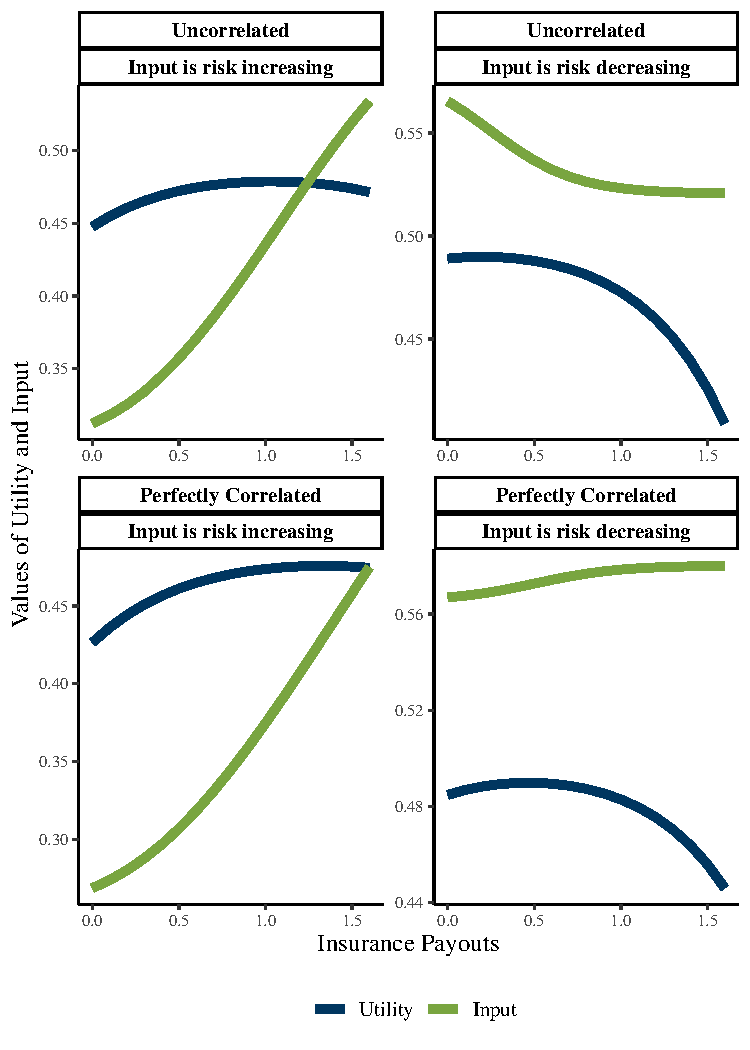
\includegraphics{ibi-behavior_files/figure-pdf/fig-iter-1.pdf}

}

\caption{\label{fig-iter}Improvements in utility (green lines) and
changes in optimal input use (blue lines) with index insurance. Shocks
are uncorrelated with high mean productivity (\(\alpha=0.75\)), high
risk aversion \(a=3\), and relatively more variable weather shocks than
biological (\(\sigma_{w}=0.4\) vs \(\sigma_{t}=0.1\))}

\end{figure}

Optimal input use changes monotonically with index insurance depending
on the risk characteristics of the input (Figure~\ref{fig-iter}). Risk
increasing inputs always increase with insurance. Risk decreasing inputs
are ambiguous following Proposition~\ref{prp-ind} and
Proposition~\ref{prp-corr}. Independent shocks lead risk decreasing
inputs to monotonically decrease with \(\omega\) contracts. Risk
decreasing inputs will monotonically raise or lower with an insurance
contract built on \(\omega\) when correlated with \(\theta\).

The concavity of utility, as demonstrated by the blue parabolas in all
panels of Figure~\ref{fig-iter}, implies there exists an optimal amount
of insurance for fishers to buy. The monotoncity of input use in all
cases suggests that the insurance level that maximizes utility will
persevere the sign of input changes. Therefore, an endogenous choice of
insurance will not affect the direction of input change, but it will
affect the magnitude.

For example, risk increasing inputs have higher levels of insurance
payouts that maximize utility. Allowing fishers to choose insurance
coverage ensures that the choice of insurance and input use changes are
welfare improving and will not bias input choices with over or under
investment of insurance. Simulations moving forward will allow fishers
to choose both inputs and insurance coverage.

Adding an endogenous to Equation~\ref{eq-maxsim} amends the choice set
in Equation~\ref{eq-maxsim2}. Furthermore, we run two groups of
simulations. One with the insurance contracted indemnified on \(\omega\)
as shown in Equation~\ref{eq-maxsim}, and another with the index built
on \(\theta\) to test all conditions of Proposition~\ref{prp-ind} and
Proposition~\ref{prp-corr}.

\begin{equation}\protect\hypertarget{eq-maxsim2}{}{
\begin{aligned}
U&\equiv\max_{x,\gamma}\mathbb{E}[u]=\mathbb{E}[(1-\exp(-a(\pi(x,\hat\beta,\theta,\omega)+\mathbb{I}(\gamma))]\\
\mathbb{I}(\gamma)&=\begin{cases}-\rho\gamma & \text{if } \omega\ge \bar\omega\\
(1-\rho)\gamma & \text{if } \omega<\bar\omega
\end{cases}
\end{aligned}
}\label{eq-maxsim2}\end{equation}

Correlation between biological and productivity risk impact optimal
choice of input in line with Proposition~\ref{prp-ind} and
Proposition~\ref{prp-corr} when contracts use \(\omega\) as the index.
Uncorrelated shocks have consistent signs of input use in accordance to
the underlying inputs risk effect function (Figure~\ref{fig-corr}).
Insurance lowers risk decreasing inputs, but at smaller margins when
productivity is high. Insurance raises risk increasing inputs at similar
margins for all levels of productivity. This result verifies
Proposition~\ref{prp-ind} for \(\omega\) index contracts.

Perfectly correlated shocks, shown by the far right cluster of bars in
each panel of Figure~\ref{fig-corr}, verify the results of
Proposition~\ref{prp-corr}. Insurance always raises risk increasing
inputs, but has ambiguous effects on risk decreasing inputs. The
tradeoff between the risk reducing capacity of the inputs and its
marginal productivity drives this result. Because the variables are
perfectly correlated, insurance protects against both biological and
production risk. Insurance decreases the need to reduce productivity
risk through \(h(x)\), but increases the desire to take on more
biological risk to achieve greater harvests. Which of these effects
dominates depends on how productive is the input. Inputs with low
productivity do not provide as much benefit when taking on further
biological risk, so fishers will decrease their use if the input is risk
decreasing. Very productive inputs provide excellent marginal returns
and it becomes worthwhile to pursue additional harvest as insurance
protects the additional risk.

The more correlated the variables, the stronger the effect. Perfectly
correlated indices imply zero basis risk and would be considered
``perfect'' contracts. The behavioral implications of our model suggest
that this form of basis risk could lead to more conservation degradation
than imperfect uncorrelated contracts. However, basis risk is a
significant impediment to insurance uptake (Binswanger-Mkhize 2012;
Clarke 2016). The average improvement in utility for contracts with high
basis risk was 1.5\%, and 7.8\% for ``perfect'' contracts implying that
fisher demand would be much higher for the perfect contract. If
policymakers want to promote well designed contracts, there must be
other considerations to curtail harvest expansion otherwise long run
sustainability will be impeded.

\begin{figure}

{\centering 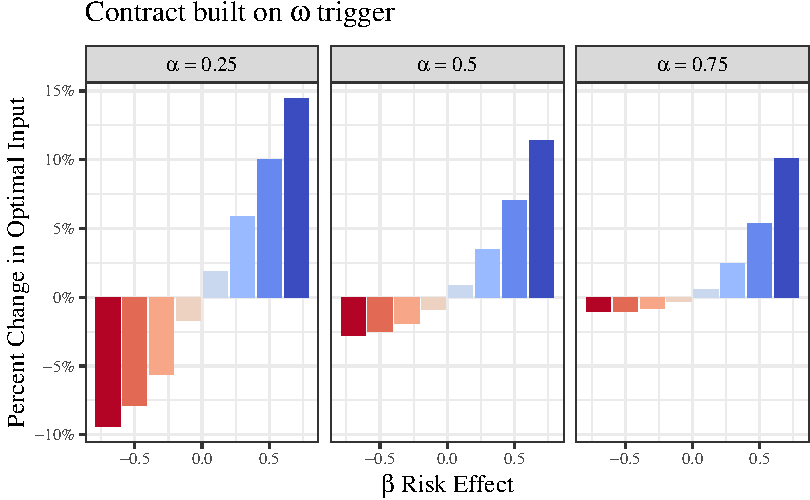
\includegraphics{ibi-behavior_files/figure-pdf/fig-corr-1.pdf}

}

\caption{\label{fig-corr}Percentage change in optimal input with an
index insurance contract using \(\omega\) as the index. Risk increasing
inputs (blue bars) always increase input use, while risk decreasing
inputs (red bars) have ambiguous effects depending on the basis risk
(correlation on the x-axis) and relative productivity of the input
(\(\alpha\) in the panels).}

\end{figure}

Figure~\ref{fig-corr-theta} verifies the remaining properties of
Proposition~\ref{prp-ind} and Proposition~\ref{prp-corr}. Contracts
built on \(\theta\) as the index show more bias towards overfishing
because of the inherent risk increasing characteristics of \(f(x)\).
Uncorrelated shocks imply that insurance will only protect shocks on
\(\theta\). Production can expand as insurance protects the additional
risk of \(\theta f(x)\) regardless of the risk decreasing inputs. The
results become ambiguous when the shocks are correlated for the same
reasons as when contracts are built on \(\omega\). The overall
protection offered by insurance will allow whichever marginal effect
between \(hx_(x)\) and \(f_x(x)\) to dominate the direction of optimal
input use.

\begin{figure}

{\centering 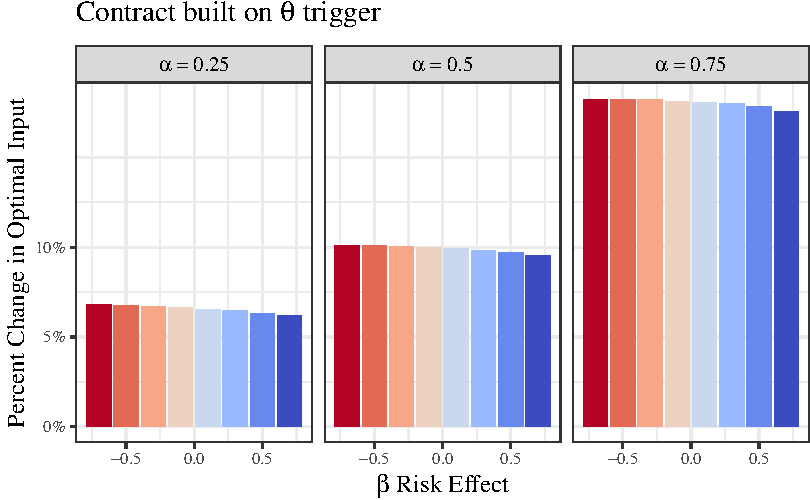
\includegraphics{ibi-behavior_files/figure-pdf/fig-corr-theta-1.pdf}

}

\caption{\label{fig-corr-theta}Percentage change in optimal input with
an index insurance contract indenmified on \(\theta\). Higher
corrleations (x-axis) lead to amiguous results where \(\omega\) risk
decreasing inputs (red bars) could lead to decreases in input use.
Panels indicate the biological production elasticity. Risk increasing
inputs (blue bars) always lead to greater input use.}

\end{figure}

Magnitude of input changes are sensitive to other parameters. More risk
averse fishers respond more aggressively to insurance and make
relatively more changes toward their input decisions (Panel A in
Figure~\ref{fig-sum}). Risk aversion implies more sensitivity towards
risk. The protection from insurance has greater marginal value for more
risk averse fishers. Greater marginal value of insurance means they can
invest less into risk reducing inputs than before, and have more
protection from greater shocks with risk increasing inputs.

Fisher input choice are much more responsive to insurance protection
from larger productivity risks (Panel B Figure~\ref{fig-sum}). Similar
to risk aversion, the greater the shocks the greater the marginal value
of insurance is to mitigate those shocks. In more volatile environments,
insurance provides significantly more income smoothing leading to
similar incentives as the higher risk aversion example.

Trigger levels do not appear to have differing impacts on input use.
Setting the trigger levels to more catastrophic coverage did not
encourage fishers to change their input use relative to the other
parameters. While necessary for applying Lemma~\ref{lem-mp} and
Lemma~\ref{lem-corr} in the proofs, the results of
Proposition~\ref{prp-ind} and Proposition~\ref{prp-corr} would appear to
hold if \(\bar\omega\ne0\).

\begin{figure}

{\centering 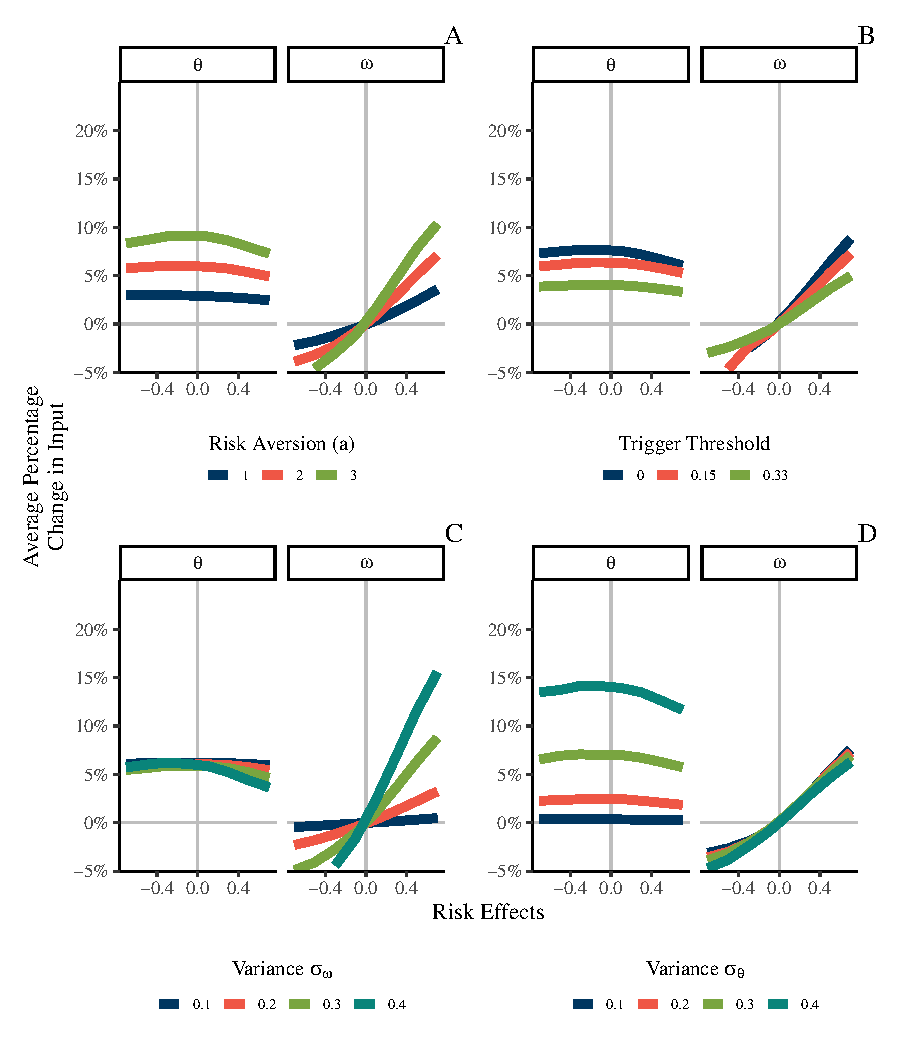
\includegraphics{ibi-behavior_files/figure-pdf/fig-sum-1.pdf}

}

\caption{\label{fig-sum}Risk Aversion (A), weather variance \(\omega\)
(B), and trigger (C) all influence the magnitude of change in harvest.
Mean production elasticity is set to 0.5. Average percent change in
input (y-axis) is summarized across all other parameter combinations for
each risk effect value of \(\beta\).}

\end{figure}

In the next section we use parameters from Asche \emph{et al.} (2020) to
calculate the overall change in harvest with multiple inputs interacting
with index insurance.

\hypertarget{application-to-norwegian-fisheries}{%
\subsection{Application to Norwegian
Fisheries}\label{application-to-norwegian-fisheries}}

Asche et al., (2020) aggregated by vessel type and not species, so there
is no reasonable estimate for biomass. They accounted for biomass using
fixed effects in their regression, but without additional information we
cannot parameterize the mean and variance of biomass. Therefore, our
simulations normalize mean biomass to 1 and we assume the biomass
shocks, \(\theta\), have three degrees of correlation with \(\omega\),
\(\{0,0.5,1\}\). Norwegian fisheries are well managed so the biological
variance could be mitigated through quota systems or accurate stock
assessments. The simulation model uses three inputs (capital \(k\),
labor \(l\), and fuel \(f\)) instead of one (Equation~\ref{eq-sim3}).

\begin{equation}\protect\hypertarget{eq-sim3}{}{
\pi(k,l,f)=k^{\alpha_k}l^{\alpha_l}f^{\alpha_f}(\hat\beta+\theta)+\omega k^{\beta_k}l^{\beta_l}k^{\beta_f}-c_kk^2-c_ll^2-c_ff^2
}\label{eq-sim3}\end{equation}

Fishers in the simulation choose inputs and insurance coverage to
maximize expected utility. We use either index as shown by \(z\).

\begin{equation}\protect\hypertarget{eq-maxasche}{}{
\begin{aligned}
U&\equiv\max_{\gamma,k,l,f}\mathbb{E}[u]=\mathbb{E}[u(k^{\alpha_k}l^{\alpha_l}f^{\alpha_f}(\hat\beta+\theta)+\omega k^{\beta_k}l^{\beta_l}k^{\beta_f}-c_kk^2-c_ll^2-c_ff^2+\mathbb{I}(\gamma)]\\
\mathbb{I}(\gamma)&=\begin{cases}-\rho\gamma & \text{if } z\ge \bar z\\
(1-\rho)z& \text{if } z<\bar z
\end{cases}
\end{aligned}
}\label{eq-maxasche}\end{equation}

Table~\ref{tbl-asche} shows the production and risk elasticities of the
four vessel types used in the simulation. While not all elasticities
were found to be statistically different from zero, we used their raw
values because dropping only those variables that are significant in
both matching parameters would have kept only a few valid combinations.
All non-significant elasticities led to small changes as expected, but
their interactions with other inputs could partially drive some of the
observed outcomes.

\hypertarget{tbl-asche}{}
\begin{longtable}[]{@{}
  >{\raggedright\arraybackslash}p{(\columnwidth - 12\tabcolsep) * \real{0.2609}}
  >{\raggedleft\arraybackslash}p{(\columnwidth - 12\tabcolsep) * \real{0.1304}}
  >{\raggedleft\arraybackslash}p{(\columnwidth - 12\tabcolsep) * \real{0.1304}}
  >{\raggedleft\arraybackslash}p{(\columnwidth - 12\tabcolsep) * \real{0.1304}}
  >{\raggedleft\arraybackslash}p{(\columnwidth - 12\tabcolsep) * \real{0.1159}}
  >{\raggedleft\arraybackslash}p{(\columnwidth - 12\tabcolsep) * \real{0.1159}}
  >{\raggedleft\arraybackslash}p{(\columnwidth - 12\tabcolsep) * \real{0.1159}}@{}}
\caption{\label{tbl-asche}Production and Risk elasticities of Norwegian
Fisheries from Asche et al., (2020)}\tabularnewline
\toprule\noalign{}
\begin{minipage}[b]{\linewidth}\raggedright
\end{minipage} & \begin{minipage}[b]{\linewidth}\raggedleft
\(\alpha_k\)
\end{minipage} & \begin{minipage}[b]{\linewidth}\raggedleft
\(\alpha_l\)
\end{minipage} & \begin{minipage}[b]{\linewidth}\raggedleft
\(\alpha_f\)
\end{minipage} & \begin{minipage}[b]{\linewidth}\raggedleft
\(\beta_k\)
\end{minipage} & \begin{minipage}[b]{\linewidth}\raggedleft
\(\beta_l\)
\end{minipage} & \begin{minipage}[b]{\linewidth}\raggedleft
\(\beta_f\)
\end{minipage} \\
\midrule\noalign{}
\endfirsthead
\toprule\noalign{}
\begin{minipage}[b]{\linewidth}\raggedright
\end{minipage} & \begin{minipage}[b]{\linewidth}\raggedleft
\(\alpha_k\)
\end{minipage} & \begin{minipage}[b]{\linewidth}\raggedleft
\(\alpha_l\)
\end{minipage} & \begin{minipage}[b]{\linewidth}\raggedleft
\(\alpha_f\)
\end{minipage} & \begin{minipage}[b]{\linewidth}\raggedleft
\(\beta_k\)
\end{minipage} & \begin{minipage}[b]{\linewidth}\raggedleft
\(\beta_l\)
\end{minipage} & \begin{minipage}[b]{\linewidth}\raggedleft
\(\beta_f\)
\end{minipage} \\
\midrule\noalign{}
\endhead
\bottomrule\noalign{}
\endlastfoot
Coastal Seiners & 0.294 & 0.421 & 0.457 & 0.184 & -0.432 & 0.119 \\
Coastal Groundfish & 0.463 & 0.421 & 0.355 & 0.965 & -0.080 & 0.113 \\
Purse Seiners & 0.941 & -0.108 & 0.605 & -0.454 & -0.231 & 0.160 \\
Groundfish Trawlers & 0.210 & 0.106 & 0.531 & -2.788 & -0.110 &
-0.024 \\
\end{longtable}

We use the same parameter space as the previous simulations to test the
sensitivity of fisher input choices with index insurance. We plot the
distribution of input change after insurance for all combinations of
parameters for each fishery in Figure~\ref{fig-asche} based on a
contract with \(\omega\) as the index. We report the highest density as
an indicator of the general direction of input change, but the
distribution shows that mixes of risk increasing and decreasing inputs
can lead to ambiguous results.

We also examine Proposition~\ref{prp-samre} by isolating the input use
change in each fishery through density plots in
Figure~\ref{fig-asche-input}.

\begin{figure}

{\centering 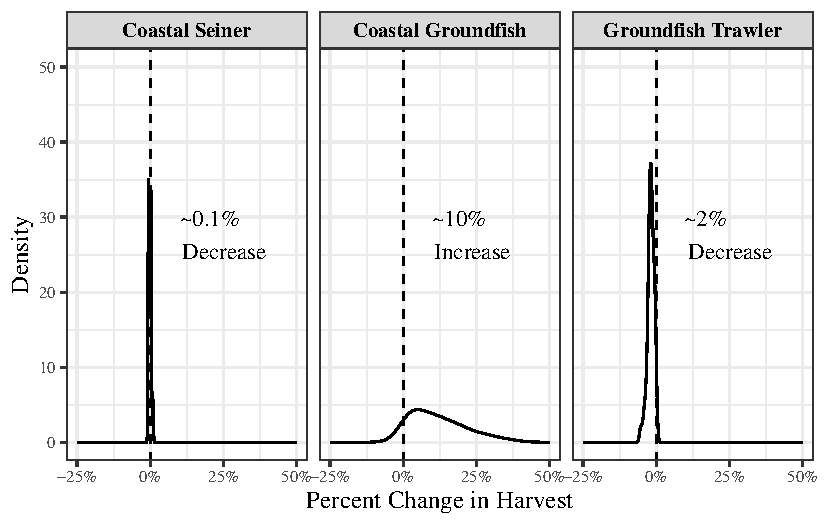
\includegraphics{ibi-behavior_files/figure-pdf/fig-asche-1.pdf}

}

\caption{\label{fig-asche}Density plots of the percent change in harvest
for each vessel type in Norwegian fisheries. The dashed line represents
no change in harvest. The text labels represent the median percent
change in harvest for each vessel type.}

\end{figure}

Overall, insurance leads to relatively small changes in harvest for all
fisheries, but increases are stronger than decreases. Coastal groundfish
see the largest and most consistent increase in harvest. Median harvest
increased by 12.5\% with a max increase of 50\%. Coastal groundfish have
the most risk increasing inputs out of the estimated fisheries. Labor is
the only risk decreasing input in the coastal groundfish fishery at a
minuscule -0.08. Coastal groundfish show a case where the conditions of
Proposition~\ref{prp-samre} do not hold. Labor always increases despite
being a risk decreasing input (Figure~\ref{fig-asche-input}). Increased
captial and fuel use contribute the most to the increased harvest.

Coastal Seiners had a relatively balanced spectrum of risk effects. The
input mix in this case led to both increases and decreases in input use,
which on net led to near zero changes in harvest. There is a slight skew
towards increased harvest, but drastically less than the coastal
groundfish fishery. Proposition~\ref{prp-samre} does hold in this
fishery as each input follows their respective increase or decrease
contingent on their risk effects (Figure~\ref{fig-asche-input}).

Deep water fleets generally saw reductions in harvest. Purse Seiners
tended to decrease harvest by 4\%. Labor is never used in the
simulations because of the negative mean productivity elasticity so it
is removed from Figure~\ref{fig-asche-input}. Capital is the most
productive input with the strongest risk effect. It appears to control
the direction of overall harvest. The conditions of
Proposition~\ref{prp-samre} do not hold as there are some parameter
combinations that lead risk decreasing capital to increase and risk
increasing fuel to lower with insurance.

Groundfish trawlers consistently see small decreases of 1.5\% in harvest
(Figure~\ref{fig-asche}). All inputs are risk decreasing with capital
having the strongest risk effect out of all inputs across all fisheries.
However, it has a relatively low marginal productivity. Insurance
decreases trawler capital use by about 8\%, but the low productivity
leads to only a 1.5\% decrease in overall harvest. Labor and fuel see
small declines in use that are always negative. When correlations are
allowed, there are some instances that see increases in harvest matching
the observations of Proposition~\ref{prp-corr}. The conditions of
Proposition~\ref{prp-samre} are met in this fishery as expected because
each input shares the same risk effect (Figure~\ref{fig-asche-input}).

\begin{figure}

{\centering 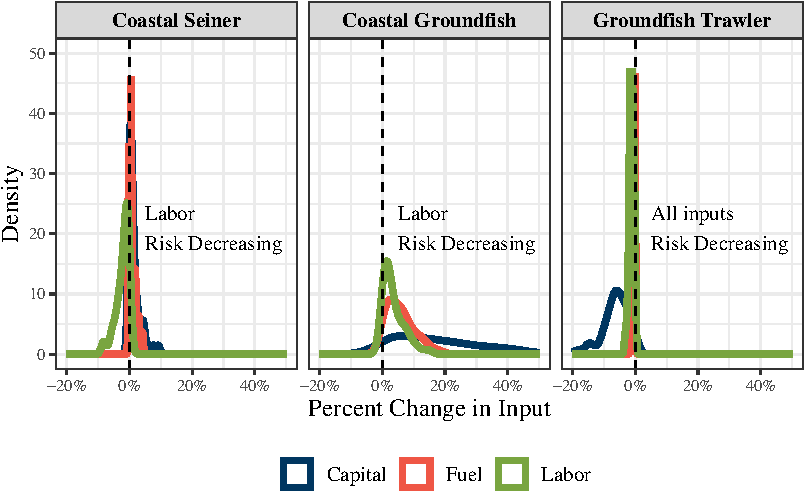
\includegraphics{ibi-behavior_files/figure-pdf/fig-asche-input-1.pdf}

}

\caption{\label{fig-asche-input}Density plots of the percent change in
input use for each vessel type in Norwegian fisheries. The dashed black
line represents no change in input use. Risk decreasing inputs are
labeled. Labor (green lines) is dropped for Purse Seiners because labor
was never used in simulations due to negative productivity elasticity.}

\end{figure}

Applying an insurance contract indemnified on \(\theta\) instead of
\(\omega\) shows similar results, but shifts the direction towards more
overfishing (Figure~\ref{fig-asche-theta}). The most prominent shifts
occur in the groundfish trawlers and coastal seiner fleets. In
Figure~\ref{fig-asche}, the percent change in harvest for coastal
seiners is indistinguishable from zero. With a \(\theta\) index
contract, there is now a pronounced shift towards overharvesting
(Figure~\ref{fig-asche-theta}).

Groundfish trawlers have opposite results with a contract indenmified on
\(\theta\). Despite the risk decreasing dominance of capital, fishers
will choose to increase production as insurance drastically protects
against the added harvest risk. This result most clearly shows the
impact of different insurance contracts and the potential for
maladatpive behavior change. Without considering all the margins for
change, insurance protecting against biological risk will still
encourage overfishing without additional constraints.

\begin{figure}

{\centering 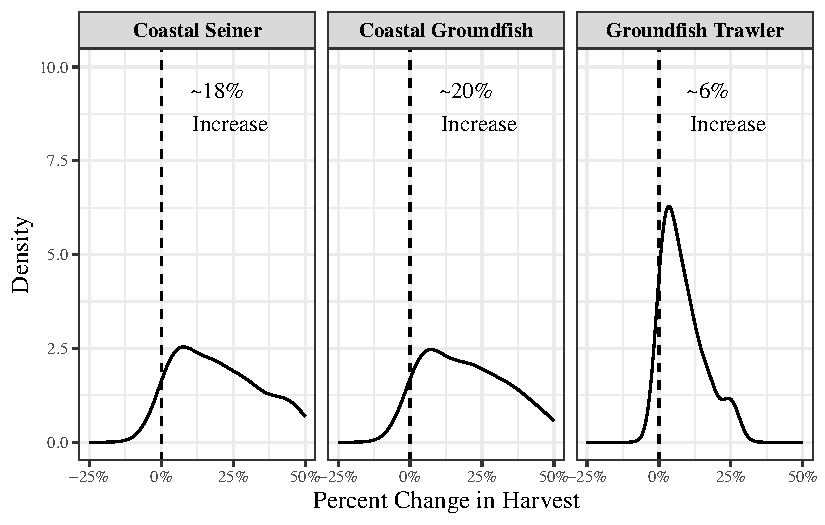
\includegraphics{ibi-behavior_files/figure-pdf/fig-asche-theta-1.pdf}

}

\caption{\label{fig-asche-theta}Density plots of the percent change in
harvest for each vessel type in Norwegian fisheries with insurance
contract indemnified on biological risk \(\theta\). The dashed line
represents no change in harvest. The text labels represent the median
percent change in harvest for each vessel type.}

\end{figure}

\hypertarget{sec-disc}{%
\section{Discussion}\label{sec-disc}}

This paper makes three distinct contributions. First, index insurance
will have behavioral impacts on fishers' input decisions, which in turn
will lead to changes in fishery sustainability. Second, the design of
index insurance contracts affects policyholder behavior contingent on
the mitigation strategies available to protect the underwritten risk.
Third, fishers face distinct sources of risk through the biology of fish
stocks and inherent harvesting variability that can be modeled with a
new stochastic production function.

The fundamental driver of fishers' behavior changes is whether the
marginal change in productivity is balanced by the marginal change in
risk. Fishers are more willing to increase production if insurance
negates the additional risk of expanded production. Since insurance
lowers risk, fishers need less self insurance through risk reducing
inputs and can reduce their overall input use. However, using less
inputs implies less catch and revenue creating a unique tension that
exists throughout the analysis. Across all simulations, decreased input
use was smaller than increased input use holding all other parameters
constant. Behavior change in fisheries will lean towards expanding
production creating a dilemma for conservation efforts.

Index insurance would improve welfare in Norwegian fisheries, but also
lead to changes in harvest that depends on the production risk effects
of fishing fleets. Coastal groundfish trawlers increased fishing
pressures by 12.5\% when offered insurance. Capital and fuel are risk
increasing inputs, and encourage the increased harvest. If an insurance
policy was applied to provide the income smoothing benefit of insurance,
the policymaker must take measures to mitigate the preserve incentive to
expand fishing production. Otherwise, the long term health of the stock
could be degraded and fishers would be worse off in the long run (Müller
\emph{et al.} 2017; John \emph{et al.} 2019; Bulte and Haagsma 2021).

Norwegian pelagic groundfish trawlers would have the opposite
considerations. When offered insurance they reduced their harvest by
1.5\%. Though small, it will lead to improved fishery sustainability.
The long term benefit of insurance would increase with improved stock
health. The decline in harvest was driven by a reduction in
overcapitalization, because capital was a significantly risk decreasing
input. Policymakers should attempt to identify fisheries with risk
decreasing input for insurance contracts to improve sustainability if
index insurance is to operate in isolation of other policies.

Ex-ante idenfication of input risk effects is challenging. Production
risk effects remain an elusive concept in fisheries, and need to
reconciled in order to articulate more accurate behavior changes of
fishery index insurance. Crop covers and pesticide provide clear
examples of risk decreasing inputs in agriculture, but what do risk
decreasing inputs look like in fisheries? Asche \emph{et al.} (2020)
provide empirical evidence of the existence of risk decreasing inputs,
but do not elaborate on why or how labor and capital directly decrease
risk. Labor is perhaps the more intuitive risk decreasing input.
Technical expertise of crew and captains can hedge against luck when
fishing (Alvarez \emph{et al.} 2006). Better trained crew can deploy
gear in a safe and timely manner, increasing the likelihood of effective
sets.

Fuel as a risk increasing input in fisheries makes intuitive sense as
well. Fuel is used to power vessels and is a direct cost of fishing.
Fishers explore productive fishing grounds for the best location. Every
hour at sea increases the harvest reward, but also the chances of
failure.

Capital is a more complex input, because it is shown to be both risk
increasing and decreasing. Capital investments in fisheries typically
refer to vessel tonnage, engine power, and gear technology. The
spatiotemporal dimension of fishing decisions may explain how capital
can potentially possess both risk effects. Fishers have to make
decisions on where, when, and how long to fish that differ from the set
grids of agriculture (Reimer \emph{et al.} 2017). Capital offers
protection from risk by allowing fishers to explore more fishing
grounds, use more secure gear, and fish in more adverse weather
conditions. When common pool resources incentivize the race to fish,
having larger vessels may be a risk reducing input as the sooner a
fisher harvests from the stock, they assure their income at the expense
of other fishers. Adding risk aversion to standard models of common pool
fisheries suggests fishers should lower their capital use compared to
risk neutral allocations (Mesterton-Gibbons 1993; Tilman \emph{et al.}
2018). Yet, overcapitalization and overfishing are more often observed
in the real world. Either fishers are never risk averse or the risk
effects of capital are not as simple as the standard model suggests.
When capital is allowed to be risk decreasing, optimal input choices are
much higher than risk neutral equilibrium suggesting fishers are making
rational, risk averse decisions even while overfishing.

Fishers exposure to multiple sources of risk further necessitates
insurance, but also makes it more challenging to design.
Proposition~\ref{prp-corr} shows the interaction between the biological
and production risk obfuscate the moral hazard of insurance. The assumed
volatility of more fish in the ocean leads the harvest function to
implicitly be risk increasing in our specification of stochastic
production. With this assumption, designing a contract around a
primarily biological shock will bias the results towards more
overfishing. In the Norwegian fisheries, contracts built on biological
risk increased median fish harvest in all fisheries. Median fish harvest
rose precipitously by 22\% in the risk increasing coastal groundfish.
One simple step for policymakers to avoid perverse moral hazards would
be to avoid index insurance contracts triggered on weather variables
that impact biomass.

However, most bioeconomic models simplify the complex effects of stock
dynamics into multiplicative forms as modeled in this paper. Instead,
different forms of risk could be embedded into the biological component
of fishery models. Stock variance could be greater in overfished stocks
instead of healthier ones, reflecting more vulnerability in weaker
states (Sims \emph{et al.} 2018). Adapting alternative, more
biologically focused specifications of biological risk could change the
behavioral effects of insurance. If insurance protects from more risk,
fishers may be more willing to expose themselves to greater risk at more
vulnerable stock levels. Alternatively, insurance could help mitigate
risk and incentivize fishers to move toward healthier stocks with less
variance by alleviating pressures to fish. Further analysis is required
to understand the full implications of biological risk effects in
fisheries.

Selecting suitable fisheries is equally as important as selecting the
right contract. Moral hazards exist and will have noticeable effects on
fishing production. Further considerations must be taken into account of
the impacts of index insurance.

The transfer between inputs and insurance reflects the substitution
between self-insurance and formal insurance (Quaas and Baumgärtner
2008). If index insurance is designed to reduce fishing capacity,
efforts must be made to ensure that it does not take away from the self
resiliency of fishers. Labor appears to be consistently risk reducing
and acts as a form of self insurance. If index insurance incentivizes
captains to hire less crew, the stock of fish may be preserved, but less
employment may reverberate throughout the community. Fishing is often a
primary employment opportunity in coastal communities. The resiliency of
the community would be compromised rather than enhanced with fewer jobs.
The same idea applies to capital. If fishers are over investing in
capital to hedge against some form of risk, policymakers need to be sure
the insurance is replacing maladaptive self insurance behavior.

The primary form of self insurance in fisheries is management. To this
point our analysis explicitly modeled scenarios without the existence of
management. Most fisheries are managed in some form. The interaction
between management and insurance may be complementary or substitutes.
For example, well managed fisheries that have responsive harvest control
rules may not need insurance. The management system is already providing
the necessary risk protection. Insurance demand and uptake may be low in
these fisheries. Insurance could instead complement management to
provide the financial relief that management cannot offer. Managers
often focus on the biological health of the fishery that can run at odds
with fishers' desires to enhance their income. Insurance can act as the
financial relief and allow managers to pursue more active strategies to
protect fish stocks without political resistance from lowered quotas.
Additionally, management can provide the constraints on insurance moral
hazard so the income smoothing benefits are passed to fishers, but not
the long term degradation. The interaction between insurance and
management requires further investigation especially with the the
numerous management strategies that exist in fisheries.

Design and access of insurance must also consider equity. The current US
federal disaster relief program is inequitable with bias towards large
industrial vessels (Jardine \emph{et al.} 2020). Creating another
program with equal inequity would be foolhardy. Current US farm
subsidies, including insurance premiums, are heavily skewed towards
large agribusinesses (White and Hoppe 2012). Dimensions of access,
procedural, representation, and distribution must all be built into the
design of new fishery index insurance programs (Fisher \emph{et al.}
2019). For example, small scale fishers may have income constraints that
prevent them from buying the initial contract. Micro-finance options
connected to insurance have been used in agriculture to alleviate this
burden with some success (Dougherty \emph{et al.} 2021). Additionally,
who receives the payouts needs thorough consideration. Payouts solely to
vessel owners may ignore support to valuable, yet vulnerable fishery
participants. Deckhands and crew are laid off during closures. If index
insurance payouts are going through the entire fishery, the most
vulnerable in the event of closures must be protected as well. Contract
stipulations could mandate that only cost expenses are covered by
payouts thereby including lost wages to the crew. Agriculture contracts
often are designed to directly cover expenses (He \emph{et al.} (2020)).
Labor expenses could be included in the contract to ensure that the crew
is protected as well.

Our model only directly models behavior change through moral hazards.
Index insurance could be designed to incentivize other forms of
sustainable behavior change. We define three pathways insurance can
change behavior: Moral hazards, Quid Pro Quo, and Collective Action.
Moral hazards were proven in this paper to have ambiguous impacts
controlled by the risk characteristics of fishery inputs. The incentives
of moral hazards will always exist, therefore other measures could be
taken to either limit the downside behavioral effects of insurance or
stimulate other forms of sustainable behavior.

Quid Pro Quo expands contract design to explicitly build in conservation
measures. Fishers would be required to adopt sustainable practices in
order to qualify for insurance. Quid Pro Quo is already used in
agricultural insurance in the form of Good Farm Practices. Farmers must
submit management plans to US Risk Management Agency that clearly
outline their conservation practices in order to qualify for insurance.
Working closely with management agencies, insurance companies could
design contracts that require fishers to follow fishery specific
management practices. For example, fishers may be incentivized to use
more sustainable gear types, have an observer onboard, or reduce
bycatch. Management input is needed to tailor fishery best practices to
insurance contracts. Further research would need to uncover the full
impact of Quid Pro Quo, but an initial hypothesis would be the fishers
will be willing to adopt sustainable practices so long as the marginal
gain in utility from the insurance is greater or equal to the necessary
sustainable changes. Otherwise fishers will not want to buy the
contracts and the insurance has no binding stipulations to change the
fishery.

Collective action ties insurance premiums to biological outcomes to
leverage the political economy of the fishery. Insures could reduce
premiums in fisheries that have robust management practices such as
adaptive harvest control rules, stock assessments, or marine protected
areas in the vicinity. Fishers could either pressure regulators to adopt
these actions or form industry groups to undertake the required actions.
Insurers would agree to this if triggers are connected to biological
health so that negative shocks are less frequent and thus payouts occur
less. Fishers gain from the reduced insurance premium and the increased
sustainability of harvest with rigorous management in place.

Ultimately, if index insurance is to be used in fisheries, it must be
designed with clear objectives and intentions. Index insurance can meet
objectives of income stability and risk reduction, but there has been an
implicit assumption by practitioners that index insurance will always
lead to improved sustainability. Without considering the behavior change
of fishers when adopting insurance, the outcomes may not be as expected.
New insights derived from this paper will help guide the efficient and
sustainable implementation of fisheries index insurance.

\newpage
\appendix
\renewcommand{\thefigure}{A\arabic{figure}}
\renewcommand{\thetable}{A\arabic{table}}
\setcounter{figure}{0}
\setcounter{table}{0}

\hypertarget{appendix}{%
\section{Appendix}\label{appendix}}

\hypertarget{proof-of-lem-mp}{%
\subsection{\texorpdfstring{Proof of
Lemma~\ref{lem-mp}}{Proof of Lemma~}}\label{proof-of-lem-mp}}

\textbf{Lemma 3.1} \emph{Individual fisher expected marginal profit of a
specific input, \(x_m\), is greater in the good state than expected
marginal profit in the bad state when \(h_{x_m}(X)>0\). Expected
marginal profit is higher in the bad state when \(h_{x_m}(X)<0\). If
\(h_{x_m}(X)=0\), the marginal profits are equivalent in both states.}

By the first order conditions, there exist optimal values of any
individual input \(x_m\) that must be chosen before the realization of
the states of the world. Therefore \(h(X^*)\), \(f(X^*)\), and
\(c(X^*)\) are equal across states.

First we prove the case when \(z\equiv\omega\). The steps and logic will
follow nearly identically for \(\theta\).

Marginal utility in both states of the world is controlled by risk
effects and the sign of the random variables. Given \(\theta\) is
independent of \(\omega\), the expected value of
\(\mathbb{E}[\theta|\omega\lessgtr\bar\omega]=0\). The difference in
expected marginal profit across insurance states is defined as:

\begin{equation}\protect\hypertarget{eq-comppi1}{}{
\begin{aligned}
\small
\frac{\partial \mathbb{E}[\pi|\omega<\bar\omega]}{\partial x^*_m}-\frac{\partial \mathbb{E}[\pi|\omega>\bar\omega]}{\partial x^*_m}=&\mathbb{E}[\omega h_{x_m^*}(X^*)|\omega<\bar\omega]+\cancel{f_{x_m^*}(X^*)\hat{B}}+\cancel{\mathbb{E}[\theta f_x(X^*)|\omega <\bar\omega]}-\cancel{c_{x^*_m}(X^*)} \\
&-\mathbb{E}[\omega h_{x_m^*}(X^*)|\omega>\bar\omega]+\cancel{f_{x_m^*}(X^*)\hat{B}}+\cancel{\mathbb{E}[\theta f_x(X^*)|\omega >\bar\omega]}-\cancel{c_{x^*_m}(X^*)}\\
=&\mathbb{E}[\omega h_{x_m^*}(X^*)|\omega<\bar\omega]-\mathbb{E}[\omega h_{x_m^*}(X^*)|\omega>\bar\omega]
\end{aligned}
}\label{eq-comppi1}\end{equation}

If an input is risk decreasing then \(h_{x_m}(X)<0\). Then
Equation~\ref{eq-comppi1} is positive and marginal profit in the bad
state is greater than the marginal profit in the good state. Adding more
of a risk reducing input reduces the negative impact in the bad state
relative to the good state.

\[
\frac{\partial \mathbb{E}[\pi|\omega<\bar\omega]}{\partial x^*_m}-\frac{\partial \mathbb{E}[\pi|\omega>\bar\omega]}{\partial x^*_m}=\overbrace{\mathbb{E}[\omega h_{x_m^*}(X^*)|\omega<\bar\omega]-\mathbb{E}[\omega h_{x_m^*}(X^*)|\omega>\bar\omega]}^{+}
\]

Repeating the same steps for risk increasing inputs \(h_{x_m}(X)>0\)
shows that marginal profit in the bad state is less than marginal profit
in the good state.

\[
\frac{\partial \mathbb{E}[\pi|\omega<\bar\omega]}{\partial x^*_m}-\frac{\partial \mathbb{E}[\pi|\omega>\bar\omega]}{\partial x^*_m}=\overbrace{\mathbb{E}[\omega h_{x_m^*}(X^*)|\omega<\bar\omega]-\mathbb{E}[\omega h_{x_m^*}(X^*)|\omega>\bar\omega]}^{-}
\]

When the insurance contract is triggered on biological risk \(\theta\),
uncorrelated shocks will always lead to higher marginal profit in the
good state. Uncorrelated shocks lead
\(\mathbb{E}[\omega|\theta \lessgtr \bar \theta]=0\).

\begin{equation}\protect\hypertarget{eq-compz}{}{
\begin{aligned}
\small
\frac{\partial \mathbb{E}[\pi|\theta<\bar\theta]}{\partial x^*_m}-\frac{\partial \mathbb{E}[\pi|\theta>\bar\theta]}{\partial x^*_m}=&\cancel{\mathbb{E}[\omega h_{x_m^*}(X^*)|\theta<\bar\theta]}+\cancel{f_{x_m^*}(X^*)\hat{B}}+\mathbb{E}[\theta f_x(X^*)|\theta <\bar\theta]-\cancel{c_{x^*_m}(X^*)} \\
&-\cancel{\mathbb{E}[\omega h_{x_m^*}(X^*)|\theta>\bar\theta]}-\cancel{f_{x_m^*}(X^*)\hat{B}}-\mathbb{E}[\theta f_x(X^*)|\theta >\bar\theta]+\cancel{c_{x^*_m}(X^*)}\\
=&\mathbb{E}[\theta f_x(X^*)|\theta <\bar\theta]-\mathbb{E}[\theta f_x(X^*)|\theta >\bar\theta]
\end{aligned}
}\label{eq-compz}\end{equation}

The concavity of \(f(X)\) leads to \(f_x(X)>0\) always.
Equation~\ref{eq-compz} can then be signed to always be negative so that
marginal profit in the good state is always higher when insurance
contracts are triggered on \(\theta\).

\[
\frac{\partial \mathbb{E}[\pi|\theta<\bar\theta]}{\partial x^*_m}-\frac{\partial \mathbb{E}[\pi|\theta>\bar\theta]}{\partial x^*_m}=\overbrace{\mathbb{E}[\theta f_{x_m^*}(X^*)|\theta<\bar\theta]-\mathbb{E}[\theta f_{x_m^*}(X^*)|\theta>\bar\theta]}^{-}
\]

\hypertarget{proof-of-lem-corr}{%
\subsection{\texorpdfstring{Proof of
Lemma~\ref{lem-corr}}{Proof of Lemma~}}\label{proof-of-lem-corr}}

Perfect correlation between two random variables centered at 0 imply
that whenever one variable is negative, so too is the other. Due to
this, we focus only on \(\omega\) as the index. The proof follows
identically if replaced by an index on \(\theta\).

\begin{equation}\protect\hypertarget{eq-corrmp}{}{
\begin{aligned}
\frac{\partial \mathbb{E}[\pi|\omega<\bar\omega]}{\partial x}-\frac{\partial \mathbb{E}[\pi|\omega>\bar\omega]}{\partial x}=\cancel{f_{x}(x)}\hat{B}+\mathbb{E}[\theta f_x(x)|\omega<\bar\omega]+\mathbb{E}[\omega h_{x}(x)|\omega<\bar\omega]-\cancel c(x)\\
-\cancel{f_{x}(x)}\hat{B}+\mathbb{E}[\theta f_x(x)|\omega>\bar\omega]+\mathbb{E}[\omega h_{x}(x)|\omega>\bar\omega]-\cancel c(x)
\end{aligned}
}\label{eq-corrmp}\end{equation}

When \(h_x(X)>0\), Equation~\ref{eq-corrmp} is always negative. Expected
marginal profit is always higher in the good trigger state when shocks
are perfectly correlated.

When \(h_x(X)<0\), Equation~\ref{eq-corrmp} is ambiguous. The sign of
each line depends on the relative effect between \(f_x(X)\) and
\(h_x(X)\). If the risk effects term dominates then
Equation~\ref{eq-corrmp} will be positive. Without further information
it is impossible to know which effect dominates.

\hypertarget{sec-partial}{%
\subsection{Partial derivatives}\label{sec-partial}}

Partial derivatives used to sign Equation~\ref{eq-ivtsol} are shown
below. For brevity, \(\pi(X,\hat B,\omega,\theta)\) is reduced to
\(\pi\).

\begin{equation}\protect\hypertarget{eq-kk}{}{
\begin{aligned}
\frac{\partial U}{\partial x_a \partial x_a}=\int^\infty_{-\infty}&\left[ \int^{\bar z_i}_{-\infty}j_{\omega,\theta}(\omega,\theta)[u''(\pi+(1-J(\bar z_i))\gamma)\frac{\partial\pi}{\partial x_a}+u'(\pi+(1-J(\bar z_i))\gamma)\frac{\partial \pi}{\partial x_a x_a}]dz_i \right. \\
&\left. +\int^\infty_{\bar z_i}j_{\omega,\theta}(\omega,\theta)[u''(\pi-J(\bar z_i)\gamma)\frac{\partial\pi}{\partial x_a}+u'(\pi-J(\bar z_i)\gamma)\frac{\partial \pi}{\partial x_a x_a}]dz_i\right]dz_r
\end{aligned}
}\label{eq-kk}\end{equation}

\begin{equation}\protect\hypertarget{eq-ll}{}{
\begin{aligned}
\frac{\partial U}{\partial x_b \partial x_b}=\int^\infty_{-\infty}&\left[ \int^{\bar z_i}_{-\infty}j_{\omega,\theta}(\omega,\theta)[u''(\pi+(1-J(\bar z_i))\gamma)\frac{\partial\pi}{\partial x_b}+u'(\pi+(1-J(\bar z_i))\gamma)\frac{\partial \pi}{\partial x_b x_b}]dz_i \right. \\
&\left.\int^\infty_{\bar z_i}j_{\omega,\theta}(\omega,\theta)[u''(\pi-J(\bar z_i)\gamma)\frac{\partial\pi}{\partial x_b}+u'(\pi-J(\bar z_i)\gamma)\frac{\partial \pi}{\partial x_b x_b}]dz_i\right]dz_r
\end{aligned}
}\label{eq-ll}\end{equation}

\begin{equation}\protect\hypertarget{eq-crossl}{}{
\begin{aligned}
\frac{\partial U}{\partial x_a \partial x_b}=\int^\infty_{-\infty}&\left[ \int^{\bar z_i}_{-\infty}j_{\omega,\theta}(\omega,\theta)[u''(\pi+(1-J(\bar z_i))\gamma)\frac{\partial\pi}{\partial x_a}\frac{\partial \pi}{\partial x_b}+u'(\pi+(1-J(\bar z_i))\gamma)\frac{\partial \pi}{\partial x_a x_b}]dz_i \right. \\
& \left.\int^\infty_{\bar z_i}j_{\omega,\theta}(\omega,\theta)[u''(\pi-J(\bar z_i)\gamma)\frac{\partial\pi}{\partial x_a}\frac{\partial \pi}{\partial x_b}+u'(\pi-J(\bar z_i)\gamma)\frac{\partial \pi}{\partial x_a x_b}]dz_i\right]dz_r
\end{aligned}
}\label{eq-crossl}\end{equation}

\begin{equation}\protect\hypertarget{eq-crossk}{}{
\begin{aligned}
\frac{\partial U}{\partial x_b \partial x_a}=\int^\infty_{-\infty}&\left[ \int^{\bar z_i}_{-\infty}j_{\omega,\theta}(\omega,\theta)[u''(\pi+(1-J(\bar z_i))\gamma)\frac{\partial\pi}{\partial x_a}\frac{\partial \pi}{\partial x_b}+u'(\pi+(1-J(\bar z_i))\gamma)\frac{\partial \pi}{\partial x_b x_a}]dz_i \right. \\
& \left.\int^\infty_{\bar z_i}j_{\omega,\theta}(\omega,\theta)[u''(\pi-J(\bar z_i)\gamma)\frac{\partial\pi}{\partial x_a}\frac{\partial \pi}{\partial x_b}+u'(\pi-J(\bar z_i)\gamma)\frac{\partial \pi}{\partial x_b x_a}]dz_i\right]dz_r
\end{aligned}
}\label{eq-crossk}\end{equation}

\begin{equation}\protect\hypertarget{eq-kgam}{}{
\begin{aligned}
\frac{\partial U}{\partial x_a \partial \gamma}=\int^\infty_{-\infty}&\left[ \int^{\bar z_i}_{-\infty}j_{\omega,\theta}(\omega,\theta)u''(\pi+(1-J(\bar z_i))\gamma)\frac{\partial\pi}{\partial x_a}(1-J(\bar z_i)dz_i \right. \\
& \left.\int^\infty_{\bar z_i}j_{\omega,\theta}(\omega,\theta)u''(\pi-J(\bar z_i)\gamma)\frac{\partial\pi}{\partial x_a}(-J(\bar z_i))dz_i\right]dz_r
\end{aligned}
}\label{eq-kgam}\end{equation}

\begin{equation}\protect\hypertarget{eq-lgam}{}{
\begin{aligned}
\frac{\partial U}{\partial x_b \partial \gamma}=\int^\infty_{-\infty}&\left[ \int^{\bar z_i}_{-\infty}j_{\omega,\theta}(\omega,\theta)u''(\pi+(1-J(\bar z_i))\gamma)\frac{\partial\pi}{\partial x_b}(1-J(\bar z_i)dz_i \right. \\
&\left.\int^\infty_{\bar z_i}j_{\omega,\theta}(\omega,\theta)u''(\pi-J(\bar z_i)\gamma)\frac{\partial\pi}{\partial x_b}(-J(\bar z_i))dz_i\right]dz_r
\end{aligned}
}\label{eq-lgam}\end{equation}

\hypertarget{sec-samre}{%
\subsection{\texorpdfstring{Proof of
Proposition~\ref{prp-samre}}{Proof of Proposition~}}\label{sec-samre}}

\begin{proof}

Lemma~\ref{lem-mp} allows us to sign the partial equations
Equation~\ref{eq-kgam} and Equation~\ref{eq-lgam} for any risk effect on
either input. Concave utility by definition leads to \(u''<0\). For
simplicity, we will only focus on
\(\frac{\partial U}{\partial x_a\partial \gamma}\), but all applies
equally to \(\frac{\partial U}{\partial x_b\partial \gamma}\). Insurance
payouts equalize profits between different states. If insurance
completely covers all loss and \(x_a\) is risk increasing, then
\(\frac{\partial U}{\partial x_a\partial \gamma}\) is positive.

\begin{equation}\protect\hypertarget{eq-kgamsol}{}{
\begin{aligned}
\frac{U}{\partial x_a \partial \gamma}=\int^{\infty}_{-\infty}&\overbrace{j_{\theta}(\theta)J(\bar\theta)(1-J(\bar\theta))u''(\theta,\cdot)}^{-}\\
&\left[ \int^{\bar\omega}_{-\infty}\underbrace{j_{\omega}(\omega)\frac{\partial \pi}{\partial x_a}d\omega
-\int^{\infty}_{\bar{\theta}}j_{\omega}(\omega)\frac{\partial \pi}{\partial x_a}d\omega}_{-}\right] d\theta\\
>0
\end{aligned}
}\label{eq-kgamsol}\end{equation}

Suppose both inputs are risk increasing so
\(\frac{\partial U}{\partial x_a\partial \gamma}\) and
\(\frac{\partial U}{\partial x_b\partial \gamma}\) are positive. The
only way for Equation~\ref{eq-ivtsol} to be unambiguously positive is
for \(\frac{\partial U}{\partial x_a\partial x_b}\) and
\(\frac{\partial U}{\partial x_a\partial x_b}\) to be positive.

\[
\begin{aligned}
&\frac{\partial x_a}{\partial \gamma}=\overbrace{\frac{-1}{Det}}^{-}\left[\overbrace{\overbrace{\frac{\partial U}{\partial x_b \partial x_b}}^{-}\overbrace{\frac{\partial U}{\partial x_a \partial \gamma}}^{+}\overbrace{-\frac{\partial U}{\partial x_a \partial x_b}}^{-}\overbrace{\frac{\partial U}{\partial x_b \partial \gamma}}^{+}}^{-}\right] >0\\
&\frac{\partial x_b}{\partial \gamma}=\overbrace{\frac{-1}{Det}}^{-}\left[\overbrace{\overbrace{\frac{-\partial U}{\partial x_b \partial x_a}}^{-}\overbrace{\frac{\partial U}{\partial x_a \partial \gamma}}^{+}+\overbrace{\frac{\partial U}{\partial x_a \partial x_a}}^{-}\overbrace{\frac{\partial U}{\partial x_b \partial \gamma}}^{+}}^{-}\right]>0
\end{aligned}
\]

Both risk increasing inputs will be raised with index insurance.
Repeating the same steps above with risk decreasing inputs shows both
inputs unambiguously decrease with index insurance.

Now suppose inputs have mixed risk effects. For simplicity, \(x_a\) will
be risk increasing and \(x_b\) will be risk decreasing. The results will
hold for the opposite case. By Lemma~\ref{lem-mp},
\(\frac{\partial U}{\partial x_a\partial \gamma}\) is positive, while
\(\frac{\partial U}{\partial x_b\partial \gamma}\) is negative.
Equation~\ref{eq-ivtsol} will be unambiguously positive if
\(\frac{\partial U}{\partial x_a\partial x_b}\) and
\(\frac{\partial U}{\partial x_b\partial x_a}\) are negative.

\[
\begin{aligned}
&\frac{\partial x_a}{\partial \gamma}=\overbrace{\frac{-1}{Det}}^{-}\left[\overbrace{\overbrace{\frac{\partial U}{\partial x_b\partial x_b}}^{-}\overbrace{\frac{\partial U}{\partial x_a \partial \gamma}}^{+}\overbrace{-\frac{\partial U}{\partial x_a \partial x_b}}^{+}\overbrace{\frac{\partial U}{\partial x_b\partial \gamma}}^{-}}^{-}\right] >0\\
&\frac{\partial x_b}{\partial \gamma}=\overbrace{\frac{-1}{Det}}^{-}\left[\overbrace{\overbrace{\frac{-\partial U}{\partial x_b\partial x_a}}^{+}\overbrace{\frac{\partial U}{\partial x_a \partial \gamma}}^{+}+\overbrace{\frac{\partial U}{\partial x_a \partial x_a}}^{-}\overbrace{\frac{\partial U}{\partial x_b\partial \gamma}}^{-}}^{+}\right]<0
\end{aligned}
\]

The risk increasing input will be raised with index insurance, while the
risk decreasing input will be lowered.

If these conditions do not hold, then it is impossible to determine
which additive element outweighs the other, and the insurance effects on
optimal input use will be ambiguous regardless of the underlying risk
effects of an input.

\end{proof}

\hypertarget{references}{%
\section*{References}\label{references}}
\addcontentsline{toc}{section}{References}

\hypertarget{refs}{}
\begin{CSLReferences}{1}{0}
\leavevmode\vadjust pre{\hypertarget{ref-Alvarez2006}{}}%
Alvarez, A., Schmidt, P., Alvarez, A. and Schmidt, P. (2006)
\href{https://doi.org/10.1007/s11123-006-0002-x}{Is skill more important
than luck in explaining fish catches?} \emph{J Prod Anal} \textbf{26},
15--25.

\leavevmode\vadjust pre{\hypertarget{ref-Asche2020}{}}%
Asche, F., Cojocaru, A.L., Pincinato, R.B.M. and Roll, K.H. (2020)
\href{https://doi.org/10.1007/s10640-019-00391-2}{Production risk in the
norwegian fisheries}. \emph{Environmental and Resource Economics}
\textbf{75}, 137--149.

\leavevmode\vadjust pre{\hypertarget{ref-Babcock1996}{}}%
Babcock, B.A. and Hennessy, D.A. (1996)
\href{https://doi.org/10.2307/1243713}{Input demand under yield and
revenue insurance}. \emph{American Journal of Agricultural Economics}
\textbf{78}, 416--427.

\leavevmode\vadjust pre{\hypertarget{ref-Barbeaux2020}{}}%
Barbeaux, S.J., Holsman, K. and Zador, S. (2020)
\href{https://doi.org/10.3389/fmars.2020.00703}{Marine heatwave stress
test of ecosystem-based fisheries management in the gulf of alaska
pacific cod fishery}. \emph{Frontiers in Marine Science} \textbf{7},
1--21.

\leavevmode\vadjust pre{\hypertarget{ref-binswanger2012}{}}%
Binswanger-Mkhize, H.P. (2012)
\href{https://doi.org/10.1080/00220388.2011.625411}{Is there too much
hype about index-based agricultural insurance?} \emph{Journal of
Development Studies} \textbf{48}, 187--200.

\leavevmode\vadjust pre{\hypertarget{ref-Bulte2021}{}}%
Bulte, E. and Haagsma, R. (2021)
\href{https://doi.org/10.1007/s10640-021-00545-1}{The welfare effects of
index-based livestock insurance: Livestock herding on communal lands}.
\emph{Environmental and Resource Economics} \textbf{78}, 587--613.

\leavevmode\vadjust pre{\hypertarget{ref-Cai2016}{}}%
Cai, J. (2016) \href{https://doi.org/10.1257/pol.20130371}{The impact of
insurance provision on household production and financial decisions}.
\emph{American Economic Journal: Economic Policy} \textbf{8}, 44--88.

\leavevmode\vadjust pre{\hypertarget{ref-Carter2017}{}}%
Carter, M., Janvry, A.D., Sadoulet, E. and Sarris, A. (2017)
\href{https://doi.org/10.1146/annurev-resource-100516-053352}{Index
insurance for developing country agriculture: A reassessment}.
\emph{Annual Review of Resource Economics} \textbf{9}, 421--438.

\leavevmode\vadjust pre{\hypertarget{ref-Cavole2016}{}}%
Cavole, L.M., Demko, A.M., Diner, R.E., et al. (2016)
\href{https://doi.org/10.5670/oceanog.2016.32}{Biological impacts of the
2013--2015 warm-water anomaly in the northeast pacific: Winners, losers,
and the future}. \emph{Oceanography} \textbf{29}, 273--285.

\leavevmode\vadjust pre{\hypertarget{ref-Cheung2021}{}}%
Cheung, W.W.L., Frölicher, T.L., Lam, V.W.Y., et al. (2021)
\href{https://www.science.org}{Marine high temperature extremes amplify
the impacts of climate change on fish and fisheries}. \emph{Sci. Adv}
\textbf{7}.

\leavevmode\vadjust pre{\hypertarget{ref-Claassen2017}{}}%
Claassen, R., Langpap, C. and Wu, J. (2017)
\href{https://doi.org/10.1093/AJAE/AAW075}{Impacts of federal crop
insurance on land use and environmental quality}. \emph{American Journal
of Agricultural Economics} \textbf{99}, 592--613.

\leavevmode\vadjust pre{\hypertarget{ref-Clarke2016}{}}%
Clarke, D.J. (2016) \href{https://doi.org/10.1257/mic.20140103}{A theory
of rational demand for index insurance}. \emph{Journal: Microeconomics}
\textbf{8}, 283--306.

\leavevmode\vadjust pre{\hypertarget{ref-Collier2009}{}}%
Collier, B., Skees, J. and Barnett, B. (2009)
\href{https://doi.org/10.1057/gpp.2009.11}{Weather index insurance and
climate change: Opportunities and challenges in lower income countries}.
\emph{Geneva Papers on Risk and Insurance: Issues and Practice}
\textbf{34}, 401--424.

\leavevmode\vadjust pre{\hypertarget{ref-Deryugina2017}{}}%
Deryugina, T. and Konar, M. (2017)
\href{https://doi.org/10.1016/j.advwatres.2017.03.013}{Impacts of crop
insurance on water withdrawals for irrigation}. \emph{Advances in Water
Resources} \textbf{110}, 437--444.

\leavevmode\vadjust pre{\hypertarget{ref-Dougherty2021}{}}%
Dougherty, J.P., Gallenstein, R.A. and Mishra, K. (2021)
\href{https://doi.org/10.1093/jafeco/ejab003}{Impact of index insurance
on moral hazard in the agricultural credit market: Theory and evidence
from ghana}. \emph{Journal of African Economies} \textbf{00}, 1--31.

\leavevmode\vadjust pre{\hypertarget{ref-Eggert2004}{}}%
Eggert, H. and Tveteras, R. (2004) Stochastic production and
heterogeneous risk preferences: Commercial fishers' gear choices.
\emph{American Journal of Agricultural Economics} \textbf{86}, 199--212.

\leavevmode\vadjust pre{\hypertarget{ref-Elabed2016}{}}%
Elabed, G. and Carter, M. (2018) Ex-ante impacts of agricultural
insurance: Evidence from a field experiment in mali.

\leavevmode\vadjust pre{\hypertarget{ref-fao2020}{}}%
FAO (2020) \href{https://doi.org/10.4060/ca9229en}{The state of world
fisheries and aquaculture 2020. Sustinability in action}. \emph{INFORM}
\textbf{32}.

\leavevmode\vadjust pre{\hypertarget{ref-fao2022}{}}%
FAO (2022) World review of capture fisheries and aquaculture insurance
2022.

\leavevmode\vadjust pre{\hypertarget{ref-Fisher2019}{}}%
Fisher, E., Hellin, J., Greatrex, H. and Jensen, N. (2019)
\href{https://doi.org/10.1111/dpr.12387}{Index insurance and climate
risk management: Addressing social equity}. \emph{Development Policy
Review} \textbf{37}, 581--602.

\leavevmode\vadjust pre{\hypertarget{ref-Goodwin2004}{}}%
Goodwin, B.K., Vandeveer, M.L. and Deal, J.L. (2004) An empirical
analysis of acreage effects of participation in the federal crop
insurance program. \emph{American Journal of Agricultural Economics}
\textbf{86}, 1058--1077.

\leavevmode\vadjust pre{\hypertarget{ref-He2020}{}}%
He, J., Zheng, X., Rejesus, R. and Yorobe, J. (2020)
\href{https://doi.org/10.1111/AGEC.12558}{Input use under
cost-of-production crop insurance: Theory and evidence}.
\emph{Agricultural Economics (United Kingdom)} \textbf{51}, 343--357.

\leavevmode\vadjust pre{\hypertarget{ref-Heck2021}{}}%
Heck, N., Beck, M.W. and Reguero, B. (2021)
\href{https://doi.org/10.1016/j.marpol.2021.104698}{Storm risk and
marine fisheries: A global assessment}. \emph{Marine Policy}
\textbf{132}, 104698.

\leavevmode\vadjust pre{\hypertarget{ref-Herrmann2004}{}}%
Herrmann, M., Greenberg, J., Hamel, C. and Geier, H. (2004)
\href{https://doi.org/10.1577/M02-086.1}{Extending federal crop
insurance programs to commercial fisheries: The case of bristol bay,
alaska, sockeye salmon}. \emph{North American Journal of Fisheries
Management} \textbf{24}, 352--366.

\leavevmode\vadjust pre{\hypertarget{ref-Holland2008}{}}%
Holland, D.S. (2008)
\href{https://doi.org/10.1086/mre.23.3.42629621}{Are fishermen rational?
A fishing expedition}. \emph{Marine Resource Economics} \textbf{23},
325--344.

\leavevmode\vadjust pre{\hypertarget{ref-horowitz1993}{}}%
Horowitz, J. and Lichtenberg, E. (1993) Insurance, moral hazard, and
chemical use in agriculture. \emph{American Journal of Agricultral
Economics} \textbf{75}, 926--935.

\leavevmode\vadjust pre{\hypertarget{ref-Jardine2020}{}}%
Jardine, S.L., Fisher, M.C., Moore, S.K. and Samhouri, J.F. (2020)
\href{https://doi.org/10.1016/j.ecolecon.2020.106691}{Inequality in the
economic impacts from climate shocks in fisheries: The case of harmful
algal blooms}. \emph{Ecological Economics} \textbf{176}.

\leavevmode\vadjust pre{\hypertarget{ref-John2019}{}}%
John, F., Toth, R., Frank, K., Groeneveld, J. and Müller, B. (2019)
\href{https://doi.org/10.1016/J.ECOLECON.2018.11.021}{Ecological
vulnerability through insurance? Potential unintended consequences of
livestock drought insurance}. \emph{Ecological Economics} \textbf{157},
357--368.

\leavevmode\vadjust pre{\hypertarget{ref-Just1978}{}}%
Just, R.E. and Pope, R.D. (1978)
\href{https://doi.org/10.1016/0304-4076(78)90006-4}{Stochastic
specification of production functions and economic implications}.
\emph{Journal of Econometrics} \textbf{7}, 67--86.

\leavevmode\vadjust pre{\hypertarget{ref-Kasperski2013}{}}%
Kasperski, S. and Holland, D.S. (2013)
\href{https://doi.org/10.1073/pnas.1212278110}{Income diversification
and risk for fishermen}. \emph{Proceedings of the National Academy of
Sciences of the United States of America} \textbf{110}, 2076--2081.

\leavevmode\vadjust pre{\hypertarget{ref-Kirkley1998}{}}%
Kirkley, J. and Strand, I.E. (1998) Characterizing managerial skill and
technical efficiency in a fishery. \emph{Journal of Productivity
Analysis} \textbf{9}, 145--160.

\leavevmode\vadjust pre{\hypertarget{ref-Kompas2004}{}}%
Kompas, T., Che, T.N. and Grafton, R.Q. (2004)
\href{https://doi.org/10.1080/0003684042000218561}{Technical efficiency
effects of input controls: Evidence from australia's banana prawn
fishery}. \emph{Applied Economics} \textbf{36}, 1631--1641.

\leavevmode\vadjust pre{\hypertarget{ref-Lichtenberg2022}{}}%
Lichtenberg, E. and Iglesias, E. (2022)
\href{https://doi.org/10.1016/j.jdeveco.2022.102883}{Index insurance and
basis risk: A reconsideration}. \emph{Journal of Development Economics}
\textbf{158}.

\leavevmode\vadjust pre{\hypertarget{ref-Mahul2001}{}}%
Mahul, O. (2001) \href{https://doi.org/10.1111/0002-9092.00180}{Optimal
insurance against climatic experience}. \emph{American Journal of
Agricultural Economics} \textbf{83}, 593--604.

\leavevmode\vadjust pre{\hypertarget{ref-Maltby2023}{}}%
Maltby, K.M., Acosta, L., Townhill, B., Touza, J., White, P. and Mangi,
S.C. (2023) \href{https://doi.org/10.1093/icesjms/fsac003}{Exploring
fishers' perceptions of index insurance and coral reef health in the
context of climate-driven changes in extreme events}. \emph{ICES Journal
of Marine Science} \textbf{80}, 2210--2221.

\leavevmode\vadjust pre{\hypertarget{ref-Merino2022}{}}%
Merino, G., Urtizberea, A., Fu, D., et al. (2022)
\href{https://doi.org/10.1016/j.fishres.2022.106478}{Investigating
trends in process error as a diagnostic for integrated fisheries stock
assessments}. \emph{Fisheries Research} \textbf{256}.

\leavevmode\vadjust pre{\hypertarget{ref-gibbons1993}{}}%
Mesterton-Gibbons, M. (1993)
\href{https://doi.org/10.1111/j.1939-7445.1993.tb00143.x}{Game-theoretic
resource modeling}. \emph{Natural Resource Modeling} \textbf{7},
93--147.

\leavevmode\vadjust pre{\hypertarget{ref-Mishra2005}{}}%
Mishra, A.K., Nimon, R.W. and El-Osta, H.S. (2005)
\href{https://doi.org/10.1016/j.jenvman.2004.08.003}{Is moral hazard
good for the environment? Revenue insurance and chemical input use}.
\emph{Journal of Environmental Management} \textbf{74}, 11--20.

\leavevmode\vadjust pre{\hypertarget{ref-muller2017}{}}%
Müller, B., Johnson, L. and Kreuer, D. (2017)
\href{https://doi.org/10.1016/j.gloenvcha.2017.06.010}{Maladaptive
outcomes of climate insurance in agriculture}. \emph{Global
Environmental Change} \textbf{46}, 23--33.

\leavevmode\vadjust pre{\hypertarget{ref-muller2011}{}}%
Müller, B., Quaas, M.F., Frank, K. and Baumgärtner, S. (2011)
\href{https://doi.org/10.1016/j.ecolecon.2011.06.011}{Pitfalls and
potential of institutional change: Rain-index insurance and the
sustainability of rangeland management}. \emph{Ecological Economics}
\textbf{70}, 2137--2144.

\leavevmode\vadjust pre{\hypertarget{ref-Murkowski2022}{}}%
Murkowski, L. (2022) Working waterfronts framework: A plan to grow and
support alaska's coastal and river communities.

\leavevmode\vadjust pre{\hypertarget{ref-Oken2021}{}}%
Oken, K.L., Holland, D.S. and Punt, A.E. (2021)
\href{https://doi.org/10.1002/eap.2307}{The effects of population
synchrony, life history, and access constraints on benefits from fishing
portfolios}. \emph{Ecological Applications} \textbf{0}, 1--16.

\leavevmode\vadjust pre{\hypertarget{ref-Outreville2014}{}}%
Outreville, J.F. (2014) Risk aversion, risk behavior, and demand for
insurance: A survey. \emph{Source: Journal of Insurance Issues}
\textbf{37}, 158--186.

\leavevmode\vadjust pre{\hypertarget{ref-Pandori2019}{}}%
Pandori, L.L.M. and Sorte, C.J.B. (2019)
\href{https://doi.org/10.1111/oik.05886}{The weakest link: Sensitivity
to climate extremes across life stages of marine invertebrates}.
\emph{Oikos} \textbf{128}, 621--629.

\leavevmode\vadjust pre{\hypertarget{ref-Pfeiffer2020}{}}%
Pfeiffer, L. (2020) \href{https://doi.org/10.1093/icesjms/fsaa145}{How
storms affect fishers' decisions about going to sea}. \emph{ICES Journal
of Marine Science} \textbf{77}, 2753--2762.

\leavevmode\vadjust pre{\hypertarget{ref-Pfeiffer2022}{}}%
Pfeiffer, L., Petesch, T. and Vasan, T. (2022)
\href{https://doi.org/10.1086/716856}{A safer catch? The role of
fisheries management in fishing safety}. \emph{Marine Resource
Economics} \textbf{37}, 1--33.

\leavevmode\vadjust pre{\hypertarget{ref-Quaas2008}{}}%
Quaas, M.F. and Baumgärtner, S. (2008)
\href{https://doi.org/10.1016/j.ecolecon.2007.07.004}{Natural vs.
Financial insurance in the management of public-good ecosystems}.
\emph{Ecological Economics} \textbf{65}, 397--406.

\leavevmode\vadjust pre{\hypertarget{ref-Ramaswami1993}{}}%
Ramaswami, B. (1993) Supply response to agricultural insurance: Risk
reduction and moral hazard effects. \emph{American Journal of
Agricultural Economics} \textbf{75}, 914--925.

\leavevmode\vadjust pre{\hypertarget{ref-RARE2021}{}}%
RARE (2021)
\href{https://rare.org/stories-articles/insuring-the-ensurers-rares-fish-forever-program-protects-the-fishers-who-feed-the-world/}{Insuring
the ensurers: A new insurance project protects the fishers who feed the
world}.

\leavevmode\vadjust pre{\hypertarget{ref-Reimer2017}{}}%
Reimer, M.N., Abbott, J.K. and Wilen, J.E. (2017)
\href{https://doi.org/10.1086/690678}{Fisheries production: Management
institutions, spatial choice, and the quest for policy invariance}.
\emph{Marine Resource Economics} \textbf{32}, 143--168.

\leavevmode\vadjust pre{\hypertarget{ref-rogers2019}{}}%
Rogers, L.A., Griffin, R., Young, T., Fuller, E., Martin, K.S. and
Pinsky, M.L. (2019)
\href{https://doi.org/10.1038/s41558-019-0503-z}{Shifting habitats
expose fishing communities to risk under climate change}. \emph{Nature
Climate Change} \textbf{9}, 512--516.

\leavevmode\vadjust pre{\hypertarget{ref-Sainsbury2019}{}}%
Sainsbury, N.C., Turner, R.A., Townhill, B.L., Mangi, S.C. and Pinnegar,
J.K. (2019) \href{https://doi.org/10.1038/s41558-019-0645-z}{The
challenges of extending climate risk insurance to fisheries}.
\emph{Nature Climate Change} \textbf{9}, 896--897.

\leavevmode\vadjust pre{\hypertarget{ref-Sethi2010}{}}%
Sethi, S.A. (2010)
\href{https://doi.org/10.1111/j.1467-2979.2010.00363.x}{Risk management
for fisheries}. \emph{Fish and Fisheries} \textbf{11}, 341--365.

\leavevmode\vadjust pre{\hypertarget{ref-Sibiko2020}{}}%
Sibiko, K.W. and Qaim, M. (2020)
\href{https://doi.org/10.1007/s12571-019-00987-y}{Weather index
insurance, agricultural input use, and crop productivity in kenya}.
\emph{Food Security} \textbf{12}, 151--167.

\leavevmode\vadjust pre{\hypertarget{ref-Sims2018}{}}%
Sims, C., Horan, R.D. and Meadows, B. (2018)
\href{https://doi.org/10.1111/NRM.12191}{Come on feel the noise:
Ecological foundations in stochastic bioeconomic models}. \emph{Natural
Resource Modeling} \textbf{31}.

\leavevmode\vadjust pre{\hypertarget{ref-Smith2023}{}}%
Smith, K.E., Burrows, M.T., Hobday, A.J., et al. (2023)
\href{https://doi.org/10.1146/annurev-marine-032122-121437}{Biological
impacts of marine heatwaves}. \emph{Annual Review of Marine Science}
\textbf{15}, 1--27.

\leavevmode\vadjust pre{\hypertarget{ref-Smith2005}{}}%
Smith, M.D. and Wilen, J.E. (2005) Heterogeneous and correlated risk
preferences in commercial fishermen: The perfect storm dilemma.
\emph{The Journal of Risk and Uncertainty} \textbf{31}, 1--53.

\leavevmode\vadjust pre{\hypertarget{ref-Smith1996}{}}%
Smith, V.H. and Goodwin, B.K. (1996)
\href{https://doi.org/10.2307/1243714}{Crop insurance, moral hazard, and
agricultural chemical use}. \emph{The Economics of Agri-Environmental
Policy} \textbf{2}, 169--179.

\leavevmode\vadjust pre{\hypertarget{ref-stoeffler2022}{}}%
Stoeffler, Q., Carter, M., Guirkinger, C. and Gelade, W. (2022)
\href{https://doi.org/10.1093/wber}{The spillover impact of index
insurance on agricultural investment by cotton farmers in burkina faso}.
\emph{The World Bank Economic Review} \textbf{36}, 114--140.

\leavevmode\vadjust pre{\hypertarget{ref-Sumaila2012}{}}%
Sumaila, U.R., Cheung, W., Dyck, A., et al. (2012)
\href{https://doi.org/10.1371/journal.pone.0040542}{Benefits of
rebuilding global marine fisheries outweigh costs}. \emph{PLoS ONE}
\textbf{7}.

\leavevmode\vadjust pre{\hypertarget{ref-sumalia2020}{}}%
Sumaila, U.R., Walsh, M., Hoareau, K., et al. (2020)
\href{https://www.oceanpanel.org/blue-}{Ocean finance: Financing the
transition to a sustainable ocean economy}.

\leavevmode\vadjust pre{\hypertarget{ref-Teh2013}{}}%
Teh, L.C.L. and Sumaila, U.R. (2013)
\href{https://doi.org/10.1111/j.1467-2979.2011.00450.x}{Contribution of
marine fisheries to worldwide employment}. \emph{Fish and Fisheries}
\textbf{14}, 77--88.

\leavevmode\vadjust pre{\hypertarget{ref-Tilman2018}{}}%
Tilman, A.R., Levin, S. and Watson, J.R. (2018)
\href{https://doi.org/10.1016/j.jtbi.2018.06.003}{Revenue-sharing clubs
provide economic insurance and incentives for sustainability in
common-pool resource systems keywords: Risk insurance social-ecological
systems fisheries management sustainability complex adaptive systems
agent-based model common-poo}. \emph{Journal of Theoretical Biology}
\textbf{454}, 205--214.

\leavevmode\vadjust pre{\hypertarget{ref-Wabnitz2019}{}}%
Wabnitz, C.C.C. and Blasiak, R. (2019)
\href{https://doi.org/10.1016/j.marpol.2019.103526}{The rapidly changing
world of ocean finance}. \emph{Marine Policy} \textbf{107}, 103526.

\leavevmode\vadjust pre{\hypertarget{ref-Watson2023}{}}%
Watson, J.R., Spillman, C.M., Little, L.R., Hobday, A.J. and Levin, P.S.
(2023) \href{https://doi.org/10.1093/icesjms/fsad175}{Enhancing the
resilience of blue foods to climate shocks using insurance}. \emph{ICES
Journal of Marine Science} \textbf{80}, 2457--2469.

\leavevmode\vadjust pre{\hypertarget{ref-White2012}{}}%
White, T.K. and Hoppe, R.A. (2012)
\href{https://www.ers.usda.gov}{Changing farm structure and the
distribution of farm payments and federal crop insurance}.

\leavevmode\vadjust pre{\hypertarget{ref-Wu2020}{}}%
Wu, S., Goodwin, B.K. and Coble, K. (2020)
\href{https://doi.org/10.1111/agec.12545}{Moral hazard and subsidized
crop insurance}. \emph{Agricultural Economics (United Kingdom)}
\textbf{51}, 131--142.

\end{CSLReferences}



\end{document}
